\documentclass[letterpaper, 10pt, conference]{ieeeconf}

% To compress the paper
%\addtolength{\textheight}{1ex}
%\addtolength{\voffset}{-.5ex}
% \renewcommand\topfraction{0.85}
% \renewcommand\bottomfraction{0.85}
% \renewcommand\floatpagefraction{0.85}

\usepackage{fixltx2e}
\usepackage[protrusion=true,expansion=true]{microtype}


\IEEEoverridecommandlockouts        % This command is only needed if you want to
                                                          % use the \thanks command
\overrideIEEEmargins
% See the \addtolength command later in the file to balance the column lengths
% on the last page of the document

%\usepackage{xparse}
\usepackage{xifthen}
\usepackage{xargs}[2008/03/08]

% Redefine citation commands compatible with natbib
\def\citep{\cite}
\def\citet{\cite}

% *** MATH PACKAGES ***
\usepackage[cmex10]{amsmath}
\interdisplaylinepenalty=2500
\usepackage{amsfonts,amssymb}

% Also, note that the amsmath package sets \interdisplaylinepenalty to 10000
% thus preventing page breaks from occurring within multiline equations. Use:
\interdisplaylinepenalty=2500
% after loading amsmath to restore such page breaks

\usepackage{bm} % for bold symbols like \bm{\alpha} or {\bm \alpha\beta}
%\usepackage{amsthm}
\usepackage{mathtools}  % Fixes and additional commands for amsmath
\usepackage{cases}  % Better than amsmath's cases environment
%\usepackage{mleftright}  % Commands \mleft and \mright

% SI Unit support: should always use to typeset numeric data
% With option per-mode=symbol: kW/s, without it: kW s^{-1}
% Quick usage:
%   \num{1+-2i}
%   \num{.3e45}
%   \SI{number}{unit} or \si{unit}
% where unit is like:
%   kg.m.s^{-1} or \kilogram\metre\per\second
%   \si[per-mode=symbol]{\kilogram\metre\per\ampere\per\second} for
%        kg m / (A s)
%\usepackage[per-mode=symbol,binary-units]{siunitx}
\usepackage[per-mode=symbol]{siunitx}


% *** GRAPHICS RELATED PACKAGES ***
%
\usepackage{graphicx}
% declare the path(s) where your graphic files are
\graphicspath{{figs/}}
% and their extensions so you won't have to specify these with
% every instance of \includegraphics
% \DeclareGraphicsExtensions{.pdf,.jpeg,.png}


% PGF/TikZ
% \usepackage{tikz}
% \usetikzlibrary{decorations,arrows,shapes,positioning}
% \usetikzlibrary{fit,backgrounds,calc}
% \usetikzlibrary{automata,matrix}
% \usetikzlibrary{circuits.logic.US,circuits.ee.IEC}
% \usetikzlibrary{shapes.geometric,shapes.symbols,shapes.arrows}

% \usepackage{pgfplots}
% \pgfplotsset{compat=newest}


% Theorem-like environments

\newtheorem{theorem}{Theorem}
\newtheorem{corollary}{Corollary}
\newtheorem{lemma}{Lemma}
\newtheorem{proposition}{Proposition}
\newtheorem{assumption}{Assumption}


% \theoremstyle{definition}
\newtheorem{definition}{Definition}
\newtheorem{problem}{Problem}

% \theoremstyle{remark}
\newtheorem{example}{Example}
\newtheorem{remark}{Remark}



% *** SPECIALIZED LIST PACKAGES ***
\usepackage{algorithm}
\usepackage{algpseudocode}  % Of the algorithmicx package, flexible, more math-like

% Define some convenient commands for algorithms
% \algnewcommand\algorithmicinput{\textbf{Input:}}
% \algnewcommand\Input{\item[\algorithmicinput]}
% \algnewcommand\algorithmicoutput{\textbf{Output:}}
% \algnewcommand\Output{\item[\algorithmicoutput]}



% *** ALIGNMENT PACKAGES ***
%
\usepackage{array}
% Frank Mittelbach's and David Carlisle's array.sty patches and improves
% the standard LaTeX2e array and tabular environments to provide better
% appearance and additional user controls. As the default LaTeX2e table
% generation code is lacking to the point of almost being broken with
% respect to the quality of the end results, all users are strongly
% advised to use an enhanced (at the very least that provided by array.sty)
% set of table tools. array.sty is already installed on most systems. The
% latest version and documentation can be obtained at:
% http://www.ctan.org/tex-archive/macros/latex/required/tools/

\usepackage{booktabs}

%\usepackage{mdwmath}
%\usepackage{mdwtab}
% Also highly recommended is Mark Wooding's extremely powerful MDW tools,
% especially mdwmath.sty and mdwtab.sty which are used to format equations
% and tables, respectively. The MDWtools set is already installed on most
% LaTeX systems. The lastest version and documentation is available at:
% http://www.ctan.org/tex-archive/macros/latex/contrib/mdwtools/


%\usepackage{eqparbox}
% Also of notable interest is Scott Pakin's eqparbox package for creating
% (automatically sized) equal width boxes - aka "natural width parboxes".
% Available at:
% http://www.ctan.org/tex-archive/macros/latex/contrib/eqparbox/




% *** SUBFIGURE PACKAGES ***
%\usepackage[font=footnotesize]{subcaption}  % For sub-figures, etc.

\usepackage[caption=false,font=footnotesize]{subfig}
% subfig.sty, also written by Steven Douglas Cochran, is the modern
% replacement for subfigure.sty.


% *** FLOAT PACKAGES ***
%
\usepackage{fixltx2e}
% fixltx2e, the successor to the earlier fix2col.sty, was written by
% Frank Mittelbach and David Carlisle. This package corrects a few problems
% in the LaTeX2e kernel, the most notable of which is that in current
% LaTeX2e releases, the ordering of single and double column floats is not
% guaranteed to be preserved. Thus, an unpatched LaTeX2e can allow a
% single column figure to be placed prior to an earlier double column
% figure. The latest version and documentation can be found at:
% http://www.ctan.org/tex-archive/macros/latex/base/



% *** PDF, URL AND HYPERLINK PACKAGES ***
%
\usepackage{url}
% url.sty was written by Donald Arseneau. It provides better support for
% handling and breaking URLs. url.sty is already installed on most LaTeX
% systems. The latest version can be obtained at:
% http://www.ctan.org/tex-archive/macros/latex/contrib/misc/
% Read the url.sty source comments for usage information. Basically,
% \url{my_url_here}.


\usepackage[reviewmark]{truonglatexdefs}


% The glossaries and acronyms
% Remove option acronym if want to combine acronyms and glossaries (terms)
% The option shortcuts allows using shortcut commands \acrs and \acrl, that
% makes it easier to switch to package acronym if necessary.
%\usepackage[nomain,nonumberlist,acronym,shortcuts,description]{glossaries}
%\makeglossaries

\usepackage{paralist}
\usepackage{todonotes}
%\newcommand{\todo}[][a]{}

\usepackage{verbatim}  % For comments

% If tikz externalization is enabled, we need to disable it just for todo notes because
% these notes use tikz, which will either cause errors or produce a lot of unnecessary files.
\ifdefined\tikzexternalenable
\makeatletter
\renewcommand{\todo}[2][]{\tikzexternaldisable\@todo[#1]{#2}\tikzexternalenable}
\renewcommand{\missingfigure}[2][]{\tikzexternaldisable\@missingfigure[#1]{#2}\tikzexternalenable}
\makeatother
\else
% If not, no need to fix.
\fi

% When I don't want to show the todo notes.
% \renewcommand{\todohilite}[1]{}
% \renewcommand{\todo}[2][]{}

% Common definitions for this paper
% Some useful math definitions, but not popular enough to be included in my official definition package.
% Copyright 2014 by Truong X. Nghiem (nghiem@seas.upenn.edu)

% \usepackage{xifthen}

%%%%%%%% Mathematical notations

\DeclareMathOperator{\diag}{diag}
\def\ones{\bm{1}}  % vector of 1's
\def\zeros{\bm{0}}  % vector of 0's
\def\IdentityMatrix{\mathbbm I}

\def\BallSet{\ensuremath{\BBBB}}  % Open ball

\DeclareMathOperator{\interior}{int}  % Interior

\DeclareMathOperator{\convhull}{co}  % Convex hull

\newcommand{\nullspace}[1]{\ensuremath{\ker\mleft(#1\mright)}}

\DeclareMathOperator{\dist}{dist}

\def\Given{\,|\,}

% This may conflict with the txfonts, pxfonts packages.
\def\coloneqq{\mathrel{\mathop:}=}
\def\definedas{\coloneqq}  % Alternatively, use \equiv for \definedas

\def\SuchThat{\,:\,}


%%%%%%%% Other definitions

\def\MATLAB{MATLAB\xspace}
\def\SIMULINK{SIMULINK\xspace}
\def\YALMIP{YALMIP\xspace}
\def\IPOPT{IPOPT\xspace}
\def\fmincon{\texttt{fmincon}\xspace}
\def\BMIBNB{BMIBNB\xspace}
\def\TrueTime{TrueTime\xspace}

%%%%%%%% Hyphenation rule
\hyphenation{MATLAB SIMULINK YALMIP IPOPT BMIBNB}

%% List of glossaries (terms) and acronyms for my thesis
% Package: glossaries.

% To define new term:
% \newglossaryentry{label}{name=actual term, sort=text-to-sort, description={long description
% of the term}, plural=special plural form}

% To define new acronym:
% \newacronym[key-val list]{label}{abbrv}{long}
% where key-val list should contain the description of the acronym (key `description' as above).
\newacronym{ODE}{ODE}{ordinary differential equation}
\newacronym{QP}{QP}{quadratic program}
\newacronym{LP}{LP}{linear program}
\newacronym{MPC}{MPC}{Model Predictive Control}
\newacronym{RHC}{RHC}{receding-horizon control}
\newacronym{DP}{DP}{Dynamic Programming}
\newacronym{CPS}{CPS}{Cyber-Physical Systems}
\newacronym{LTI}{LTI}{linear-time invariant}
\newacronym{SoC}{SoC}{state of charge}
\newacronym{EV}{EV}{electric vehicle}
\newacronym{HES}{HES}{hybrid energy systems}

%%% Local Variables: 
%%% mode: latex
%%% TeX-master: "acc14"
%%% End: 
  % The list of glossaries

% Clever references -- SHOULD BE LOADED LAST
% Generic commands: \cref and \Cref
% Seems incompatible with `algorithmic' from algorithms bundle, but can be used with `algorithmicx' (e.g. `algpseudocode').
\usepackage[capitalise]{cleveref}
\newcommand{\vref}[1]{\cref{#1}}
% When using \namecref, cleveref capitalizes the first character if the option capitalise is used, which I don't want.  So use \lcnamecref instead.

\newcommand{\figref}[1]{\cref{fig:#1}}
\renewcommand{\eqref}[1]{\cref{eq:#1}}
\newcommand{\algoref}[1]{\cref{algo:#1}}
\newcommand{\thmref}[1]{\cref{thm:#1}}
\newcommand{\secref}[1]{\cref{sec:#1}}

\newcommandx\sDelay[1][usedefault, addprefix=\global, 1=]{\delta_{#1}}
\newcommandx\sAccu[1][usedefault, addprefix=\global, 1=]{\epsilon_{#1}}


\global\long\def\XSet{\SSS}
\global\long\def\USet{\UUU}
\global\long\def\WSet{\WWW}
\global\long\def\WhSet{\widehat{\WSet}}
\global\long\def\ESet{\EEE}
\global\long\def\MPCProb#1{\PP_{#1}}
\global\long\def\ZSet{\ZZZ}
\global\long\def\Nom#1{\overbar{#1}}



%%% Local Variables: 
%%% mode: latex
%%% TeX-master: "CDC14_Anytime_Main"
%%% End: 


% correct bad hyphenation here
%\hyphenation{op-tical net-works semi-conduc-tor}

%
% \LARGE \bf
%\title{Co-design of Anytime Computation and Control for Cyber Physical Systems}
%\title{Robust Model Predictive Control of Cyber Physical Systems with Anytime Estimation}
%\title{Co-design of Anytime Estimation and Control for Cyber Physical Systems}
\title{Robust Model Predictive Control with Anytime Estimation}

\author{Truong~X.~Nghiem, Yash~V.~Pant and Rahul~Mangharam \\
Department of Electrical and Systems Engineering\\ University of Pennsylvania
\\ \{nghiem, yashpant, rahulm\}@seas.upenn.edu %
\thanks{This work was supported by STARnet -- a Semiconductor Research Corporation program sponsored by MARCO and DARPA -- and %also funded 
by the US Department of Transportation University Transportation Center Program.}
%\thanks{This material is based upon work supported by the DoE Energy Efficient Buildings (EEB) HUB sponsored by the U.S. Department of Energy under Award Number DE-EE0004261.}}
}


\begin{document}
%\bstctlcite{IEEEexample:BSTcontrol}
\maketitle

\begin{abstract}
With an increasing autonomy in modern control systems %a developing trend is that there is a a huge
comes an increasing amount of sensor data to be processed, leading to overloaded computation and communication in the systems.
For example, a vision-based robot controller processes large image data from cameras at high frequency to observe the robot's state in the surrounding environment, which is used to compute control commands.
In real-time control systems where large volume of data is processed for feedback control, the data-dependent state estimation can become a computation and communication bottleneck, resulting in potentially degraded control performance.
%Consequently, designs of such systems where either speed or accuracy of the estimator is the main criteria and this can result in degraded control performance in many cases.
Anytime algorithms, which offer a trade-off between execution time and accuracy of computation, can be leveraged in such systems.
We present a Robust Model Predictive Control approach with an Anytime State Estimation Algorithm, % for closed loop control in overloaded systems. Our control algorithm
which computes both the optimal control signal for the plant and the (time-varying) deadline/accuracy constraint for the anytime estimator.
Our approach improves the system's performance (concerning both the control performance and the estimation cost) over conventional controllers, which are designed for and operate at a fixed computation time/accuracy setting.
We numerically evaluate our approach in an idealized motion model for navigation with both state and control constraints.
\end{abstract}

\section{Introduction}
\section{Motivation}
\label{sec:motivation}
Real-time control of autonomous vehicles requires the processing of a large amount of sensor data, which is used by the vehicle to determine its position in the world and to calculate its next move.
Examples include data from cameras, LIDAR, radars and ultrasound radars, and possibly information communicated by other vehicles or the road infrastructure.
Google's autonomous vehicles generate over 750MB/s of sensor data ~\cite{diamandis2015bold} which must be processed by the perception pipeline fast enough with run-to-completion algorithms. 
To guarantee safety and meet the driving performance requirements, such run-to-completion algorithms require the hardware to be over-engineered for the worst-case: i.e., it always executes the software as if the worst-case conditions hold.
This leads to a requirement of over 4KW in computational power. 
This is a significant drain on the vehicle's lithium-ion battery capacity, which is 24kWh in a Nissan Leaf for example, and a significant percentage of the power drawn by the drive motors, which is 30kW in a small electric vehicle modeled in ADVISOR \cite{nreladvisor}.
%Note that over the past few decades, the power consumption of processors has increased by more than double, while battery energy density has only improved by about a quarter \cite{Lahiri}. 

The usage of \emph{anytime perception algorithms} allows us to perform a trade-off between the computation time of the algorithms, their power consumption, and the quality of their output.
An anytime algorithm has a pre-defined set of interruption times. 
The earlier the algorithm is interrupted, the less power it consumes, but the worse is the quality of its output in general. 
On the other hand, that quality may be sufficient for the control algorithm to achieve its goal \emph{in the current circumstances}.
For example, in this paper, the control objective is to follow the center of a driving lane, and control performance is measured by the deviation from that center.
At slow speeds, poor quality of position estimate may be tolerated since it won't lead to excessive deviations from the center.
Therefore, the perception algorithm might be interrupted early thus saving on computation power, \emph{provided it gives a good enough estimate of position. }

In \cite{RTSS15} we proposed a way in which a standard perception algorithm can be turned into an anytime algorithm via off-line profiling, and thus can offer a time/power/quality trade-off.
We also designed a model predictive controller than can make use of the trade-off offered by the anytime perception algorithm.
To achieve the time/power/quality trade-off, we produced multiple versions of the perception algorithm.
Broadly speaking, a version that ran for longer produced a higher quality output. 

In this work, we turn our attention to the time/power trade-off \emph{for a fixed quality of output} and how it can be achieved using \emph{platform-level} optimizations.
Even when the output quality is fixed, the computation delay (equivalently, throughput) is known to affect control performance. 
Thus in this paper, we study how platform-level optimizations affect the computation throughout and power, and how to use this trade-off to save computation power without overly degrading throughput.

Note that the study of how computation delay affects control performance, and the design of anytime perception and control algorithms for power saving, are not specific to autonomous vehicles.
Other control systems can benefit from these trade-offs, especially power-limited consumer robots.
In this paper, we illustrate our approach on an autonomous car $1/10^{th}$ the size of a regular car (Fig. \ref{fig:traxxas}), which uses Vanishing Point navigation \cite{VP1}. 
The setup, including the navigation algorithm, are presented in Section \ref{sec:problemSetup}.
Section \ref{sec:twoStage} describes the offline profiling of Vanishing Point, which gives us Throughput versus Power curves for various processor frequencies and various scheduling of the navigation code on CPU and GPU.
In Section \ref{sec:evaluation} we combine power and throughput into one objective function, and design a supervisor what will determine the frequency and CPU/GPU allocation to maximize the objective.
Section \ref{sec:simResults} presents experimental results that demonstrate the effect of the trade-off on control performance.
\begin{figure}[t]
	\centering
	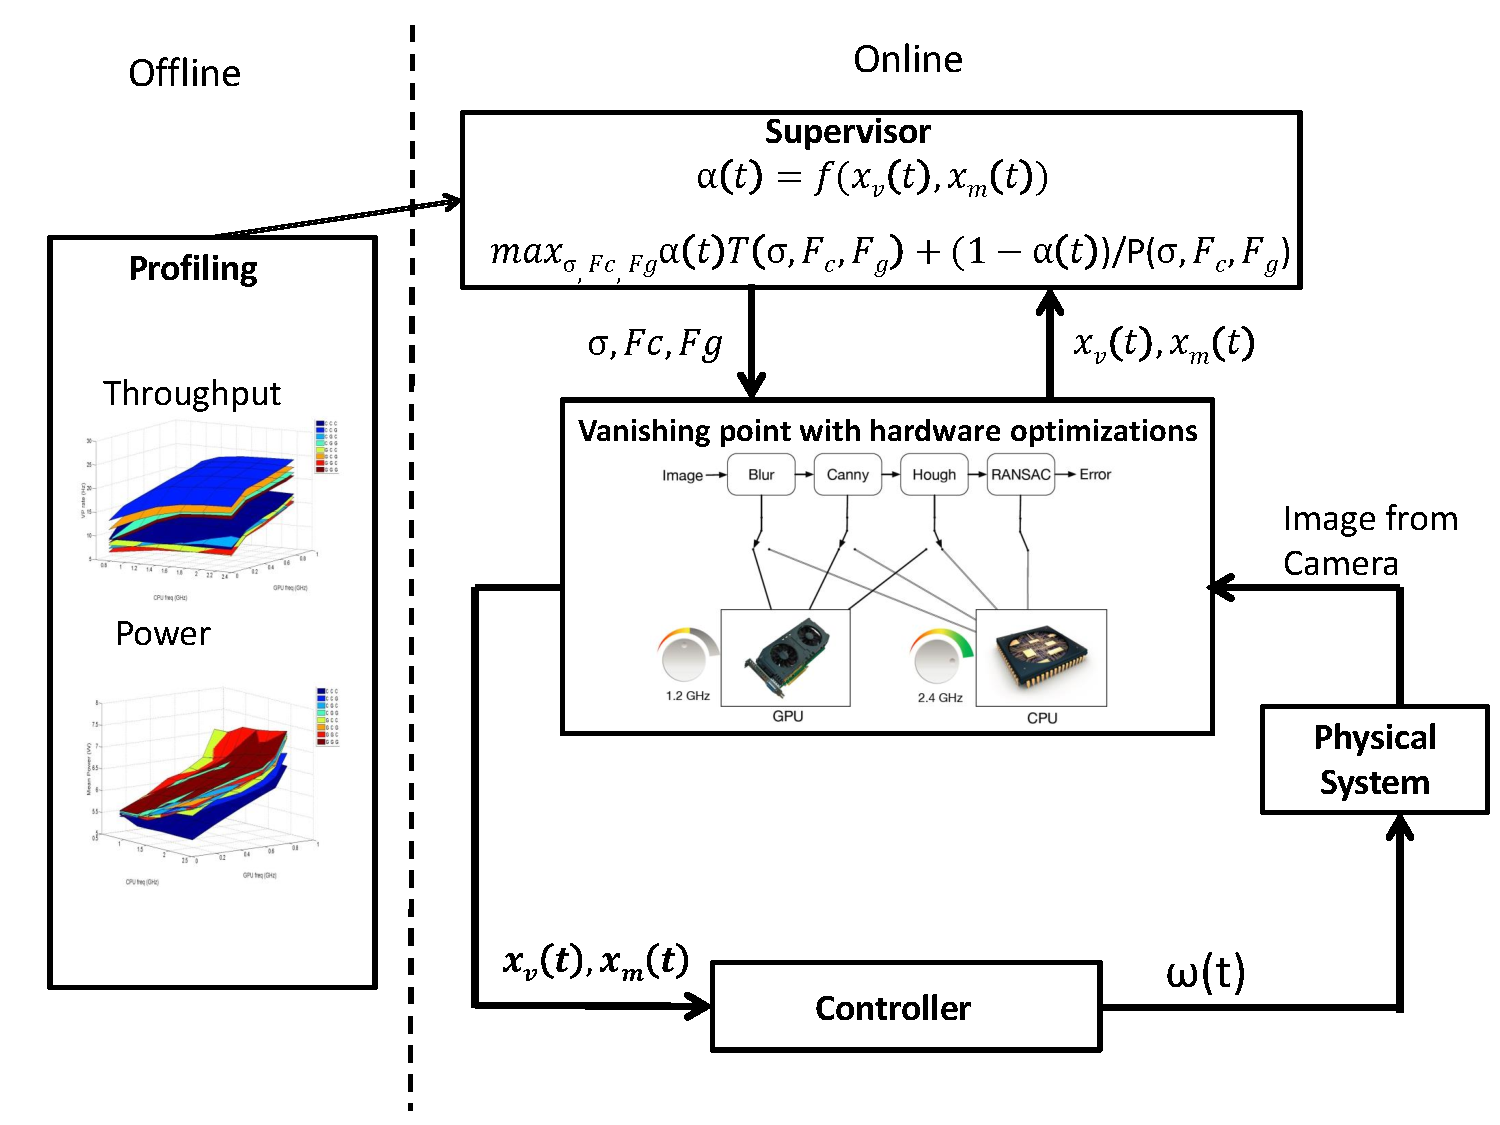
\includegraphics[width=0.46\textwidth]{Figs/bigFig.pdf}
	\caption{Two stage approach.}
	\label{fig:juicyj}%same freq diff assignment}
\end{figure} 



\section{Related Work} \label{sec:related}
%The term ``Anytime algorithm'' was introduced by Dean and Boddy\cite{boddy} in their work on time-dependent planning during the late 1980's. Horvitz\cite{horvitz} introduced the flexible computing model for time-critical decision making and planning algorithms in Artificial Intelligence. Following this, several studies in the AI community focused on composing anytime algorithms to more complex systems for sensor interpretation and path planning\cite{zilberstein, planningalgorithms}, search\cite{maxim},  and evaluation of belief networks~\cite{wellman}.

%paraphrase

Dean and Boddy \cite{boddy} introduced the term ``Anytime algorithm'' in the late 1980s. In \cite{horvitz}, Horvitz et al. introduced the flexible computing model for time-critical decision making and planning algorithms in Artificial Intelligence. Anytime algorithms for sensor interpretation and path planning in more complex systems were studied in \cite{zilberstein, planningalgorithms}. Anytime algorithms have also been studied for graph search \cite{maxim}, evaluation of belief networks \cite{wellman} and GPU architectures \cite{RTSSanytime}.

As overloaded real-time systems are becoming increasingly common, anytime algorithms for control have become a topic of research interest. Most notably, Quevedo and Gupta \cite{sequence}, Bhattacharya and Balas \cite{balas}, and Fontanelli et al. \cite{fontanelli} have contributed on the topic. In \cite{sequence}, the authors presented an algorithm that computes control input sequences for time steps into the future when given processor availability and use the previously computed inputs when there is no processor availability.
In \cite{fontanelli}, a switching condition was developed to switch among multiple feedback controllers with different worst case execution times for a single plant.
The authors in \cite{balas} proposed a methodology to get reduced order controllers with different computation requirements for a given linear time invariant (LTI) plant and a switching scheme to chose which controller to use.

Our approach differs significantly from these works as the anytime computation assumption is on the state estimator and our controller is a robust controller which can switch between different modes of the anytime estimator.
Also, while most of these works require either access to the full state of the system or have a fast estimator giving them the state estimate \cite{balas}, our algorithm accounts for the computation time/error of the estimation algorithm.
Furthermore, an advantage of the proposed RMPC is that it can handle both state and input constraints.
However, our RMPC formulation differs from related RMPC formulations \cite{chiscietal01swp,richardsetal05rmp} as it can work with time-varying error bound and execution time (delay) of the state estimator.


%%% Local Variables: 
%%% mode: latex
%%% TeX-master: "CDC14_Anytime_Main"
%%% End: 


\section{System Model} \label{sec:model}
%\section{System Model}

The control system consists of three interconnected components as
illustrated in \figref{actual-system-diagram}:
\begin{enumerate}
\item The \emph{plant} is a continuous time LTI system of the form
\begin{align}
\dot{x}(t) & =A_{c}x(t)+B_{c}u(t)+w_{c}(t)\label{eq:plant-cont-model}
\end{align}
where $x\in\RR^{n}$ is the state, $u\in\RR^{m}$ is the control input,
and $w_{c}\in\RR^{n}$ is the process noise. 
\begin{comment}
The matrices $A_{c}$
and $B_{c}$ are system matrices of appropriate dimensions. Though
the process noise \end{comment}
Though $w_{c}$ is unknown, we assume that it belongs to
a known compact and convex constraint set $\WSet_{c}\subset\RR^{n}$.
%
\item The \emph{estimator} observes the plant output $y(t)=Cx(t)+v(t)$ (where $v$ is the output noise) and estimates the current state of the plant, which cannot be measured directly. %Here $C$ is the output matrix and $v$ is the output noise.
  Let $\hat{x}(t)$ denote the estimated state at time $t$ and $e(t)=x(t)-\hat{x}(t)$ be the error between the actual and estimated states. Note that $e(t)$ is unknown, however, depending on the characteristics of the estimation algorithm, it would be bounded. The upper bound $\sAccu(t)$ of the norm $\norm{e(t)}$, where $\norm{\cdot}$ is any vector norm, determines the \emph{accuracy} of the state estimation.
  The set of error vectors corresponding to an accuracy $\sAccu\geq0$ is denoted by $\ESet(\sAccu)\definedas\{e\in\RR^{n}\SuchThat\norm{e}\leq\sAccu\}$.  We assume that the estimator is an \textit{anytime algorithm} where there is a trade-off between the accuracy and the computation time.
  In particular, the more accurate the estimation is the longer it takes to compute, and conversely.
  The accuracy of the estimator, hence its computation time, can be adjusted online by changing its parameters or its algorithm.
  % The computation time, hence the accuracy of such an algorithm can be adjusted online.

%The accuracy of
%the estimator, hence its computation time, can be adjusted online
%by changing its parameters or its algorithm.

\item The \emph{controller} computes the control input for the plant as well as
adapts the estimator's accuracy to achieve a predefined control goal.
\end{enumerate}

\begin{figure}[tb]
	\centering
		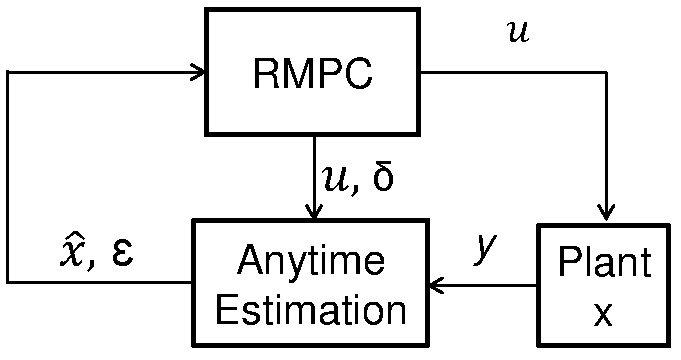
\includegraphics[width=0.40\textwidth,height=30mm]{figs/ControlFigure_scissored.pdf}
	\caption{Structure of the control and anytime estimation system.}
	\label{fig:actual-system-diagram}
\end{figure}



We consider a discrete time implementation of the controller and the estimator, in which the output $y(t)$ is sampled periodically at instants $t_{s,k}=kT$,
where $k\in\ZZplus$ and $T>0$ is a predefined sampling period.
The sampled output is fed to the estimator which computes the state
estimate $\hat{x}_{k}\definedas\hat{x}(t_{s,k})$ with the desired
accuracy $\sAccu[k]\definedas\sAccu(t_{s,k})$ determined by the controller
in the previous time step. The controller then uses this state estimate
to compute the control input $u_{k}$ as well as decide on the desired
state estimate's accuracy $\sAccu[k+1]$ for the next step. Let $\sDelay[k]$
be the worst-case total execution time of both the estimator and the
controller corresponding to the accuracy $\sAccu[k]$ of the state
estimation at time step $t_{s,k}$. We make the following theoretical
assumption of the state estimator.
\begin{assumption}
The estimation algorithm is given with a finite set of $p>0$ modes
(or options) $\Delta=\left\{ \left(\sDelay[i],\sAccu[i]\right)\right\} _{i=1}^{p}$;
each mode corresponds to a pair of time delay and estimation accuracy.
In each time step $k$, one of the estimation modes is selected, that
is $\left(\sDelay[k],\sAccu[k]\right)\in\Delta$.
\end{assumption}

This assumption means that in this paper we will not design nor analyze
the estimation algorithm; in other words, the estimator is a black-box
given to us with known characteristics. 

Furthermore, the control implementation
is subject to the following assumption.
\begin{assumption}
[Time-triggered actuation]The control actuation is delayed by $\sDelay[k]$,
\ie the control input computed by the controller is applied exactly
at the actuation instant $t_{a,k}=t_{s,k}+\sDelay[k]$.
\end{assumption}

The order of sensing\textendash{}computing\textendash{}actuating and
their timing are illustrated in the diagram in \figref{timing-diagram}.
We remark that in each step $k\geq0$, the estimation accuracy $\sAccu[k]$
and hence the delay $\sDelay[k]$ are already decided in the previous
step and known to the controller. The previous control input $u_{k-1}$
is still used until $t_{a,k}$ when the new control input $u_{k}$
is computed and applied by the controller. The controller also chooses
the next desired accuracy $\sAccu[k+1]$ and delay $\sDelay[k+1]$
to be used in the next step $k+1$. In the first step $k=0$, the
initial accuracy $\sAccu[0]$, the initial delay $\sDelay[0]$, and
the initial control input $u_{-1}$ are chosen by the designer.


\begin{figure}[tb]
	\centering
		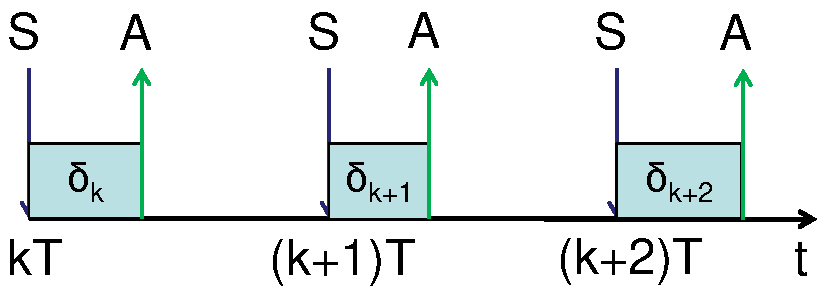
\includegraphics[width=0.45\textwidth,height=24mm]{figs/Timing_Diag.pdf}
	\caption{Timing diagram of Control with Anytime Estimation.  The symbols S and A signify the instants of (periodic) sensing and actuation respectively.}
	\label{fig:timing-diagram}
\end{figure}




\subsection{Discrete-time System Dynamics}

The plant's state at each sampling time $t_{s,k}$ can be described
by the discrete-time system:
\begin{equation}
x_{k+1}=Ax_{k}+B_{1}(\sDelay[k])u_{k-1}+B_{2}(\sDelay[k])u_{k}+w_{k}, k\geq0\label{eq:disc-dynamics} %deleted \qquad from infront of k\geq0
\end{equation}
in which
\begin{gather*}
A=\eu^{A_{c}T}, \quad
w_{k}%=\int_{t_{s,k}}^{t_{s,k+1}}\eu^{A_{c}(t_{s,k+1}-t)}w_{c}(t)\diff t \nonumber \\
=\int_{0}^{T}\eu^{A_{c}(T-t)}w_{c}(t_{s,k}+t)\diff t \\
B_{1}(\sDelay[k])%=\int_{t_{s,k}}^{t_{a,k}}\eu^{A_{c}(t_{s,k+1}-t)}B_{c}\diff t
\!=\!\int_{0}^{\sDelay[k]}\eu^{A_{c}(T-t)}B_{c}\diff t,\,
B_{2}(\sDelay[k])%=\int_{t_{a,k}}^{t_{s,k+1}}\eu^{A_{c}(t_{s,k+1}-t)}B_{c}\diff t
\!=\!\int_{\sDelay[k]}^{T}\eu^{A_{c}(T-t)}B_{c}\diff t \text.
\end{gather*}
Here $w_{k}$ is the accumulated process noise during the interval.
Because $w_{c}(t)$ is constrained in the compact and convex set $\WSet_{c}$
and $T$ is finite, we can find a compact and convex set $\WSet$
that bounds $w_{k}$, namely
\begin{equation}
w_{k}\in\WSet\qquad\forall k\geq0\text{.}\label{eq:disturb-constraint}
\end{equation}
%We remark 
Note that both the current control $u_{k}$ and the previous
control $u_{k-1}$ appear %in the dynamics 
in \eqref{disc-dynamics}.
Furthermore, the input matrices $B_{1}(\sDelay[k])$ and $B_{2}(\sDelay[k])$
depend on the delay $\sDelay[k]$; hence $\sDelay[k]$ is also an
input to the dynamics. The estimation accuracy $\sAccu[k]$ does not
appear in the equation because it only affects the state estimate
$\hat{x}_{k}$ %which is
used by the controller to compute $u_{k}$;
therefore $\sAccu[k]$ indirectly affects the dynamics via the control
input.


\subsection{State and Control Constraints}

For every step $k\geq0$, the actual state of the plant $x_{k}\definedas x(t_{s,k})$
must satisfy a safety condition that 
\begin{equation}
x_{k}\in\XSet\label{eq:state-constraint}
\end{equation}
where $\XSet\subset\RR^{n}$ is the set of safe states. We assume
that $\XSet$ is a polytope of the form $\XSet\definedas\{ x\in\RR^{n}\SuchThat Hx\leq b\} $,
where matrix $H$ and vector $b$ constitute an H-representation
of $\XSet$.
Note that $\XSet$ is not necessarily bounded. In addition, a control
input $u_{k}$ is only valid if it belongs to the predefined set of
admissible control inputs $\USet\subseteq\RR^{m}$ %, that is
\begin{equation}
u_{k}\in\USet\qquad\forall k\geq0\text{.}\label{eq:input-constraint}
\end{equation}
The sets $\XSet$ and $\USet$ are part of the problem statement and
are either chosen by the designer or determined by physical constraints
of the plant and the actuators.


\subsection{Control Performance}

The goal of the controller is two fold: it needs to maintain the state
and control constraints while minimizing a cost function given by
\(
J=\sum_{k=0}^{\infty}\left(\ell(x_{k},u_{k})+\pi(\sDelay[k])\right)
\),
where $\ell(\cdot)$ is the stage cost function for the state and
control, and $\pi(\cdot)$ is the stage cost function for the estimation
and computation.
\begin{comment}
  Typically a longer execution time $\sDelay[k]$ will
  result in a higher computation cost $\pi(\sDelay[k])$. For example,
  if the state estimation involves capturing an image by a camera then
  detecting and locating an object from the image, a longer
  computation time might correspond to a higher resolution of the
  image, more data to be transmitted and processed, and more power
  consumed for communication and computation.
\end{comment}
These stage cost functions are chosen by the designer to achieve a desired control performance.


\subsection{Control Problem}

The control problem is stated as follows.
\begin{problem}\itshape
\label{prob:control-problem}Design a feedback controller, which computes
the admissible control input $u_{k}\in\USet$ and the required estimation
accuracy $\sAccu[k+1]$ (equivalently the delay $\sDelay[k+1]$) based
on the current state estimate $\hat{x}_{k}$, to minimize the cost
$J$ while maintaining the state constraint $x_{k}\in\XSet$ for all
$k\geq 0$.
\end{problem}

\subsection{Notations}

In the rest of this paper, we use the following notational convention.
We write $x_{j\Given k}$ for a variable $x$ at time step $j$ in
the RMPC optimization for time step $k\leq j$ (\ie the prediction
made at time step $k$ of variable $x$ at time step $j$). To emphasize
that this variable depends on an independent variable $v$ we write
$x_{j\Given k}(v)$; however in cases when the dependency is implicitly
understood, we only write $x_{j\Given k}$ for brevity.
We use $\IdentityMatrix_{n}$ to denote the identity matrix of size
$n\times n$. The notation $\bm{0}_{n}$ ($\bm{1}_{n}$) represents
the column vector of length $n$ whose elements are all 0's (respectively
1's). Similarly, $\bm{0}_{n\times m}$ ($\bm{1}_{n\times m}$) is
the matrix of size $n\times m$ whose elements are all 0's (1's).
When the dimensions of the vectors or matrices are obvious
from the context, we drop the subscripts for brevity.

%%% Local Variables: 
%%% mode: latex
%%% TeX-master: "CDC14_Anytime_Main"
%%% End: 


\section{Robust MPC with Anytime Estimation}
\label{sec:RMPC}%change section name?

In this appendix we give the detailed mathematical derivation of the results of Section \ctrlProbSecRef.
The controller is designed using a Robust Model Predictive
Control (RMPC) approach via constraint restriction \cite{richardsetal05rmp, chiscietal01swp}, 
and augments it by an adaptation to the error-delay curve of the estimator.
In order to ensure robust safety and feasibility, the key idea of
the RMPC approach is to tighten the constraint sets iteratively to account
for possible effect of the disturbances. 
As time progresses, this ``robustness
margin'' is used in the MPC optimization with the nominal dynamics,
i.e., the original dynamics where the disturbances are either removed
or replaced by nominal disturbances.
%An advantage of this approach is that, 
Because only the nominal dynamics are used, the complexity of the optimization is the same as for the nominal problem.

Since the controller only has access to the estimated state $\hat{x}$, we need
to rewrite the plant's dynamics with respect to $\hat{x}$. 
The error
between $ $$x_{k}$ and $\hat{x}_{k}$ is $e_{k}=x_{k}-\hat{x}_{k}$.
At time step $k+1$ we have
\begin{align*}
\hat{x}_{k+1} & =x_{k+1}-e_{k+1}\\
 & =Ax_{k}+B_{1}(\sDelay_k)u_{k-1}+B_{2}(\sDelay[k])u_{k}+w_{k}-e_{k+1}\text{,}
\end{align*}
 then, by writing $x_{k}=\hat{x}_{k}+e_{k}$, we obtain the dynamics
\begin{equation}
\hat{x}_{k+1}=A\hat{x}_{k}+B_{1}(\sDelay[k])u_{k-1}+B_{2}(\sDelay[k])u_{k}+\hat{w}_{k}\label{eq:estimator-dynamics}
\end{equation}
 where $\hat{w}_{k}=w_{k}+Ae_{k}-e_{k+1}$.
The set of possible values of $\hat{w}_{k}$
depends on the estimation accuracy at steps $k$ and $k+1$ and is
denoted by $\hWc(\sAccu[k],\sAccu[k+1])$, i.e.,
$\hWc(\sAccu,\sAccu')\defeq \left\{ w+Ae-e'\sut w\in\Wc,e\in\ESet(\sAccu),e'\in\ESet(\sAccu')\right\}$.
Note that %we assume
$\hWc(\sAccu[k],\sAccu[k+1])$ is independent
of the time step $k$. %
It can be computed as $\hWc(\sAccu,\sAccu')=\Wc\oplus A\ESet(\sAccu)\oplus\left(-\ESet(\sAccu')\right)$
where the symbol $\oplus$ denotes the Minkowski sum of two sets.

The dynamics in \eqref{eq:estimator-dynamics} has a non-standard form
where it depends on both the current and the previous control inputs.
However we can expand the state variable to store the previous control
input as
\[
\hat{z}_{k}=\begin{bmatrix}\hat{x}_{k}\\
u_{k-1}
\end{bmatrix}\in\Re^{n+m}
\]
and rewrite the dynamics as, for all $k\geq0$,
\begin{equation}
\hat{z}_{k+1}=\hat{A}(\sDelay_k)\hat{z}_{k}+\hat{B}(\sDelay_k)u_{k}+\hat{F}\hat{w}_{k}\text{.}\label{eq:estimator-std-dynamics}
\end{equation}
Here, the system matrices are
\begin{equation}
\begin{gathered}
\hat{A}(\sDelay_k)=\begin{bmatrix}A & B_{1}(\sDelay_k)\\
\bm{0}_{m\times n} & \bm{0}_{m\times m}
\end{bmatrix},\\
\hat{B}(\sDelay_k)=\begin{bmatrix}B_{2}(\sDelay_k)\\
\IdentityMatrix_{m}
\end{bmatrix},\quad\hat{F}=\begin{bmatrix}\IdentityMatrix_{n}\\
\bm{0}_{m\times n}
\end{bmatrix}\text{.}
\end{gathered}
\label{eq:lifted-matrices}
\end{equation}

Let the actual expanded state be $z_{k}=\left[x_{k}^{T},u_{k-1}^{T}\right]^{T}$.
Because the expanded state consists of both the plant's state and
the previous control input, the state constraint $x_{k}\in\stSet$
and the control constraint $u_{k}\in\inpSet$ are equivalent to the
joint constraint $z_{k}\in\stSet\times\inpSet$. We can now describe
the RAMPC algorithm for the dynamics in \eqref{eq:estimator-std-dynamics}.

\subsection{Tractable RAMPC Algorithm}

Let $N\geq1$ be the horizon length of the RMPC optimization. 
Because the system
matrices in the state equation~(\ref{eq:estimator-std-dynamics})
depend nonlinearly on the variables $\sDelay_k$, the RMPC optimization
is generally a mixed-integer nonlinear program, which is very hard
to solve. To simplify the RMPC optimization to make it tractable, we fix the estimation mode for the entire RMPC horizon.

Let $\RAMPCProb{\de}{k}$
denote the RMPC optimization problem at step $k\geq0$ where the current
state estimate is $\hat{x}_{k}$, the current estimation mode is $(\sDelay_k,\sAccu_k)\in\Delta$,
the previous control input is $u_{k-1}$, and the estimation mode
for the entire horizon (after step $k$) is fixed at $(\sDelay,\sAccu)\in\Delta$.
Since the system matrices become constant now, if the stage cost $\ell(\cdot)$
is linear or positive semidefinite quadratic, each optimization problem
$\RAMPCProb{\de}{\cdot}$ is tractable and can be solved
efficiently as we will show later. 
The RAMPC algorithm with Anytime Estimation is stated in Alg. \algoref.


\section{Robust MPC Formulation}
\label{sec:RMPC-Formulation}
\subsection{RMPC Formulation}

We formulate the RMPC optimization $\RAMPCProb{\de}{k}$
with respect to the nominal dynamics, which is the original dynamics
in \eqref{estimator-std-dynamics} but the disturbances are either
removed or replaced by nominal disturbances. 
To ensure robust feasibility
and safety, the state constraint set is tightened after each step
using a candidate stabilizing state feedback control, and a terminal
constraint is derived. 
In this RMPC formulation, we extend the approach
in \cite{richardsetal05rmp, chiscietal01swp}. 
At time step $k$, given
$(\hat{x}_{k},\sDelay_k,\sAccu_k,u_{k-1})$ and for a fixed $(\sDelay,\sAccu)$,
we solve the following optimization 

\begin{subequations}
	\label{eq:RMPC1}
 \begin{equation} J_{\sDelay,\sAccu}^{*} \left(\hat{x}_{k},\sDelay_k,\sAccu_k,u_{k-1}\right) = \min_{\boldsymbol{u},\boldsymbol{x}}\sum_{j=0}^{N}\ell(\Nom x_{k+j\Given k},u_{k+j\Given k})
 \end{equation}
 \begin{equation}
  \text{subject to, }\forall j\in\left\{ 0,\dots,N\right\} \nonumber 
 \end{equation}
 \begin{equation}
  \Nom z_{k+j+1\Given k}=\hat{A}(\sDelay_{k+j\Given k})\Nom z_{k+j\Given k}+\hat{B}(\sDelay_{k+j\Given k})u_{k+j\Given k}\label{eq:RMPC1-dyn}
 \end{equation}
 \begin{equation}
  ( \sDelay_{k+j+1\Given k},\sAccu_{k+j+1\Given k} ) \!=\! (\sDelay,\sAccu ) \nonumber
 \end{equation}
 \begin{equation}
  (\sDelay_{k\Given k},\sAccu_{k\Given k}) \!=\! (\sDelay_k,\sAccu_k)  \label{eq:RMPC1-delay}
 \end{equation}
 \begin{equation}
  \Nom x_{k+j\Given k}=\begin{bmatrix}\IdentityMatrix_{n} \quad \bm{0}_{n\times m}\end{bmatrix}\Nom z_{k+j\Given k}\label{eq:RMPC1-z2x}
 \end{equation}
 \begin{equation}
  \Nom z_{k\Given k}=\left[\hat{x}_{k}^{T},u_{k-1}^{T}\right]^{T} \label{eq:RMPC1-z0}
 \end{equation}
 \begin{equation}
  \Nom z_{k+j\Given k}\in\ZSet_{j}\left(\sAccu_k,\sAccu\right)\label{eq:RMPC1-zset}
 \end{equation}
 \begin{equation}
  \Nom z_{k+N+1\Given k}\in\ZSet_{f}\left(\sAccu_k,\sAccu\right) \label{eq:RMPC1-zfinalset}
  \end{equation}
\end{subequations} 

in which $\Nom z$ and $\Nom x$
are the variables of the nominal dynamics. The constraints of the
optimization are explained below.
\begin{itemize}
\item \eqref{eq:RMPC1-dyn} is the nominal dynamics.
\item \eqref{eq:RMPC1-delay} states that the estimation mode is fixed at $\left(\sDelay,\sAccu\right)$
except for the first time step when it is $\left(\sDelay_k,\sAccu_k\right)$.
\item \eqref{eq:RMPC1-z2x} extracts the nominal state $\Nom x$ of the plant
from the nominal expanded state $\Nom z$.
\item \eqref{eq:RMPC1-z0} initializes the nominal expanded state at time step
$k$ by stacking the current state estimate and the previous control
input.
\item \eqref{eq:RMPC1-zset} tightens the admissible set of the nominal expanded
states by a sequence of shrinking sets.
\item \eqref{eq:RMPC1-zfinalset} constrains the terminal expanded state to
the terminal constraint set $\ZSet_{f}$.
\end{itemize}

\noindent\textit{The state constraint $\ZSet_{j}$:}
%
The tightened state constraint sets $\ZSet_{j}\left(\sAccu_k,\sAccu\right)$
are parameterized with two parameters $\sAccu_k$ and $\sAccu$.
They are defined as follows, for all $j\in\left\{ 0,\dots,N\right\} $
\begin{eqnarray}
\ZSet_{0}(\sAccu_k,\sAccu)=\ZSet\ominus\hat{F} \ESet(\sAccu_k)\label{eq:RMPC1-Z0}
\\
\ZSet_{j+1}(\sAccu_k,\sAccu)=\ZSet_{j}(\sAccu,\sAccu)\ominus L_{j}\hat{F}\hWc(\sAccu_k,\sAccu)\label{eq:RMPC1-Zj}
\label{eq:RMPC1-Z}
\end{eqnarray} 
in which the symbol $\ominus$
denotes the Pontryagin difference between two sets. The set $\ZSet$
combines the constraints for both the plant's state and the control
input: $\ZSet=\stSet\times\inpSet$. The matrix $L_{j}$ is the state
transition matrix for the nominal dynamics in \eqref{eq:RMPC1-dyn} under
a candidate state feedback gain $K_{j}(\sDelay)$, for $j\in\left\{ 0,\dots,N\right\}$
\begin{eqnarray}
\label{eq:RMPC1-L}
L_{0}=\IdentityMatrix\label{eq:RMPC1-L0}\\
L_{j+1}=(\hat{A}(\sDelay)+\hat{B}(\sDelay)K_{j}(\sDelay))L_{j}\label{eq:RMPC1-Lj}
\end{eqnarray}
Note that the possibly time-varying sequence $K_{j}(\sDelay)$ is designed for each choice of $\sDelay$ (i.e., the system matrices $\hat{A}(\sDelay)$ and $\hat{B}(\sDelay)$), hence $L_{j}$ depends on $\sDelay$; however we write $L_{j}$ for brevity. The candidate control $K_{j}(\sDelay)$ is designed to stabilize the nominal system (\ref{eq:RMPC1-dyn}), desirably as fast as possible so that the sets $\ZSet_{j}$ are shrunk as little as possible. In particular, if $K_{j}(\sDelay)$ renders the nominal system nilpotent after $M<N$ steps then $L_{j}=\bm{0}$ for all $j\geq M$, therefore $\ZSet_{j}\left(\sAccu_k,\sAccu\right)=\ZSet_{M}\left(\sAccu_k,\sAccu\right)$ for all $j>M$.


\noindent\textit{The terminal constraint $\ZSet_{f}$:}
%
$\ZSet_{f}$ is given by %the Pontryagin difference
\begin{equation}
\label{eq:RMPC1-Zf}
\ZSet_{f}\left(\sAccu_k,\sAccu\right)=\Cc(\sDelay,\sAccu)\ominus L_{N}\hat{F}\hWc(\sAccu_k,\sAccu)
\end{equation}
where $\Cc(\sDelay,\sAccu)$ is a robust control invariant admissible
set for $\sDelay$ \cite{kerrigan00rcs}, i.e., there exists a feedback control law $u=\kappa(z)$
such that $\forall z\in\Cc(\sDelay,\sAccu)$ and $\forall w\in\hWc(\sAccu,\sAccu)$
\begin{eqnarray}
\label{eq:RMPC1-Zf-invariant}
& \hat{A}(\sDelay)z \!+\! \hat{B}(\sDelay)\kappa(z) \!+\! L_{N}\hat{F}w\in\Cc(\sDelay,\sAccu) \label{eq:RMPC1-Zf-invariant-dyn}\\
& z\in\ZSet_{N}\left(\sAccu,\sAccu\right)\label{eq:RMPC1-Zf-invariant-z}
\end{eqnarray}
We remark that $\Cc(\sDelay,\sAccu)$ does not depend on $\left(\sDelay_k,\sAccu_k\right)$, therefore it can be computed offline for each mode $\left(\sDelay,\sAccu\right)$.


\section{Implementation Details} \label{sec:implementation}
Efficient computation of the constraint sets necessary for the RMPC formulation can be achieved for some special cases of disturbances and estimation errors as explained below.

\subsection{Compute State Constraint Sets}
\label{sec:ComputePontryagin}

If the error set $\ESet$ and the disturbance set $\WSet$ are defined
by vector norms, while the other sets are polytopes in H-representation
form, then it is possible to compute the Pontryagin difference in
the above equations efficiently \cite{setcomp}.%. See excerpts in \secref{Excerpts}.
\begin{itemize}
\item If $\ESet(\sAccu)\definedas\left\{ e\in\RR^{n}\SuchThat\norm{e}_{p}\leq\sAccu\right\} $
for some norm $p\in\left\{ 1,2,\infty\right\} $ then its support function
is $h_{\sAccu}(\eta)=\sAccu\norm{\eta}_{q}$ with $p^{-1}+q^{-1}=1$.
Similarly we also have $h_{w}(\eta)$.
\item Suppose $\ZSet=\left\{ z\SuchThat H_{\ZSet}z\leq b_{\ZSet}\right\} $
is a polytope in H-representation form (\ie intersection of a finite number
of half-planes). The rows of $H_{\ZSet}$ are $H_{\ZSet,i}^{T}$.
% \end{itemize}
% Then we can compute the constraint sets of the RMPC optimization efficiently.
%For example, to compute the shrinking state constraint sets in \eqref{RMPC1-Z}:
%\noindent\textit{Using \eqref{RMPC1-Z}:}
%\begin{itemize}
\item The most demanding computation in computing the constraint sets of the RMPC optimization is the Pontryagin difference.  If a set $V$ has support function $h_{V}$ then $\ZSet \ominus V$ can be computed as:
\begin{equation*}
      \ZSet \ominus V
      =\left\{ z\SuchThat H_{\ZSet}z\leq b_{\ZSet} -
       \begin{bmatrix}h_{V}\left(H_{\ZSet,1}\right)\\
         \vdots\\
         h_{V}\left(H_{\ZSet,m}\right)
       \end{bmatrix}\right\} 
 \end{equation*}
%
\item The support function $h_{\sAccu[k],\sAccu}$ for $\WhSet\left(\sAccu[k],\sAccu\right)$ is
\begin{equation*}
h_{\sAccu[k],\sAccu}(\eta)=h_{w}(\eta)+h_{\sAccu[k]}\left(A^{T}\eta\right)+h_{\sAccu}\left(-\eta\right)
\end{equation*}
%
% \item Compute 
%   \begin{equation*}
%     \begin{split}
%      \ZSet_{0}\left(\sAccu[k],\sAccu\right) 
%      &=\ZSet\ominus\hat{F}\ESet\left(\sAccu[k]\right) \\
%      &=\left\{ z\SuchThat H_{\ZSet}z\leq b_{\ZSet} -
%        \begin{bmatrix}h_{\sAccu[k]}\left(H_{\ZSet,1}\right)\\
%          \vdots\\
%          h_{\sAccu[k]}\left(H_{\ZSet,m}\right)
%        \end{bmatrix}\right\} 
%    \end{split}
%  \end{equation*}
%
% \item It is straightforward to show that
% \begin{equation*}
% \ZSet_{j}\left(\sAccu,\sAccu\right)= z\SuchThat H_{\ZSet}z\leq b_{\ZSet}-\begin{bmatrix}h_{\sAccu}\left(H_{\ZSet,1}\right)\\
% \vdots\\
% h_{\sAccu}\left(H_{\ZSet,m}\right)
% \end{bmatrix} \\
% -\sum_{i=0}^{j-1}\begin{bmatrix}h_{\sAccu,\sAccu}\left(\left(L_{j}\hat{F}\right)^{T}H_{\ZSet,1}\right)\\
% \vdots\\
% h_{\sAccu,\sAccu}\left(\left(L_{j}\hat{F}\right)^{T}H_{\ZSet,m}\right)
% \end{bmatrix}
% \end{equation*}
%
% \item Then we can compute
% %\begin{align}
% {\footnotesize
% \begin{equation}
% \begin{split}
% &\ZSet_{j+1}\left(\sAccu[k],\sAccu\right) =\ZSet_{j}\left(\sAccu,\sAccu\right)\ominus L_{j}\hat{F}\WhSet\left(\sAccu[k],\sAccu\right)\\
% &= z\SuchThat H_{\ZSet}z\leq b_{\ZSet}-\begin{bmatrix}h_{\sAccu}\left(H_{\ZSet,1}\right)\\
% \vdots\\
% h_{\sAccu}\left(H_{\ZSet,m}\right)
% \end{bmatrix} \\
% &-\sum_{i=0}^{j-1}\begin{bmatrix}h_{\sAccu,\sAccu}\left(\left(L_{i}\hat{F}\right)^{T}H_{\ZSet,1}\right)\\
% \vdots\\
% h_{\sAccu,\sAccu}\left(\left(L_{i}\hat{F}\right)^{T}H_{\ZSet,m}\right)
% \end{bmatrix}-\begin{bmatrix}h_{\sAccu[k],\sAccu}\left(\left(L_{j}\hat{F}\right)^{T}H_{\ZSet,1}\right)\\
% \vdots\\
% h_{\sAccu[k],\sAccu}\left(\left(L_{j}\hat{F}\right)^{T}H_{\ZSet,m}\right)
% \end{bmatrix}%\right\} 
% %\end{align}
% \end{split}
% \end{equation}
% }
\end{itemize}

\begin{comment}
\noindent\textit{Using \eqref{RMPC2-Yj-tight}:}
\begin{itemize}
\item We first derive the support function $h_{\YYY,j}$ of $\YYY_{j}\left(\sAccu[k],\sAccu\right)$:
%\[
{\footnotesize
\begin{equation}
h_{\YYY,j}\left(\eta\right)=\begin{cases}
h_{\sAccu[k]}\left(\begin{bmatrix}\IdentityMatrix_{n} & \bm{0}_{m}\end{bmatrix}\eta\right) & \text{\text{\text{if \ensuremath{j=0}}}}\\
\sum_{i=1}^{j}h_{w}\left(\left(\Phi^{j-i}\hat{F}\right)^{T}\eta\right)\\
+h_{\sAccu[k]}\left(\left(\Phi^{j-1}\hat{F}A\right)^{T}\eta\right)\\ +\sum_{i=2}^{j}h_{\sAccu}\left(\left(-\Phi^{j-i}\hat{B}K_{x}\right)^{T}\eta\right) & \text{if \ensuremath{j\geq1}}
\end{cases}
\end{equation}
}
%\]

\item And $Z_{j}$ can be computed as:
\[
\ZSet_{j}\left(\sAccu[k],\sAccu\right)=\left\{ z\SuchThat H_{\ZSet}z\leq b_{\ZSet}-\begin{bmatrix}h_{\YYY,j}\left(H_{\ZSet,1}\right)\\
\vdots\\
h_{\YYY,j}\left(H_{\ZSet,m}\right)
\end{bmatrix}\right\} 
\]

\end{itemize}
\end{comment}

The computation of $Z_{j}$ therefore involves only simple linear
algebra: matrix and vector multiplications, additions and substractions,
as well as vector norms. It is not difficult to see that we can write
\begin{equation}
\ZSet_{j}\left(\sAccu[k],\sAccu\right)=\left\{ z\SuchThat H_{\ZSet}z\leq b_{\ZSet}-\sAccu d_{j}-\sAccu[k]g_{j}\right\} \label{eq:impl-Zj-linear}
\end{equation}
where $d_{j}$ and $g_{j}$ are constant vectors, % whose elements are non-negative.
%Note that $d_{j}$ and $g_{j}$ 
which depend only on $\sDelay$. %
%the estimation mode $\left(\sDelay,\sAccu\right)$.
Therefore we can improve %the performance of
these computations further by pre-computing offline
these vectors; then once $\sAccu[k]$ is given, we can compute $Z_{j}$
in real time very fast.
%
The terminal set $Z_{f}$ can be computed in the same way.


\subsection{Compute Robust Control Invariant Set}

To compute the set $\CCC\left(\sDelay,\sAccu\right)$ in \eqref{RMPC1-Zf-invariant}:
\begin{enumerate}
\item Compute $\Omega=\ZSet_{N}\left(\sAccu,\sAccu\right)$ and
$\WhSet\left(\sAccu,\sAccu\right)$ (see above).
\item Call the Matlab Invariant Set Toolbox \cite{invset} to compute the maximal robust
control invariant set $\CCC\left(\sDelay,\sAccu\right)$ inside $\Omega$ subject to the disturbance
set $\WhSet\left(\sAccu,\sAccu\right)$. 
% We note that the control
% input is implicitly constrained via the constraint on the expanded
% state $z$, therefore we do not need to specify the input constraint
% explicitly (though we can use $\USet$ if we want).
\end{enumerate}


%%% Local Variables: 
%%% mode: latex
%%% TeX-master: "CDC14_Anytime_Main"
%%% End: 


%\section{Necessary Feasibility Condition for RMPC} \label{sec:necessary}
%
If any of the constraint sets in the RMPC optimization~\eqref{RMPC1}
is empty then clearly the optimization is infeasible. Therefore a
necessary feasibility condition for $\MPCProb{\sDelay,\sAccu}(\hat{x}_{k_{0}},\sDelay[k_{0}],\sAccu[k_{0]},u_{k_{0}-1})$
is that all the constraint sets are non-empty. As we have shown in
\secref{implementation}, particularly in \eqref{impl-Zj-linear},
for each $\left(\sDelay,\sAccu\right)$, these sets depend linearly
on $\sAccu[k]$. It follows that for each mode $\left(\sDelay,\sAccu\right)$,
there exists a threshold $\gamma_{\sDelay,\sAccu}$ such that if $\sAccu[k]\geq\gamma_{\sDelay,\sAccu}$
then $\MPCProb{\sDelay,\sAccu}(\hat{x}_{k_{0}},\sDelay[k_{0]},\sAccu[k_{0]},u_{k_{0}-1})$
is infeasible; in other words, $\sAccu[k]<\gamma_{\sDelay,\sAccu}$
is necessary for $\MPCProb{\sDelay,\sAccu}(\hat{x}_{k_{0}},\sDelay[k_{0]},\sAccu[k_{0]},u_{k_{0}-1})$
to be feasible. This threshold can be computed by solving the following
feasibility problem derived from the RMPC optimization
\begin{align*}
 & \gamma_{\sDelay,\sAccu}=\max\sAccu[k]\\
 & \text{subject to, }\forall j\in\left\{ 0,\dots,N\right\} \\
 & \sAccu[k]\geq0\\
 & z_{j}\in\ZSet_{j}\left(\sAccu[k],\sAccu\right)\\
 & z_{N+1}\in\ZSet_{f}\left(\sAccu[k],\sAccu\right)
\end{align*}
 which is a linear program due to the linear dependency of the constraint
sets on $\sAccu[k]$. If this LP is infeasible or $\gamma_{\sDelay,\sAccu}=0$
then this mode $\left(\sDelay,\sAccu\right)$ is invalid and needs
to be removed from $\Delta$. Because of the robust feasibility of
the RMPC optimization (\thmref{robust-feasible-RMPC}), if mode $\left(\sDelay,\sAccu\right)$
is valid we must have that 
\begin{equation}
\sAccu<\gamma_{\sDelay,\sAccu}\text{.}\label{eq:necessary-threshold-self-loop}
\end{equation}
 

A consequence of this necessary feasibility condition is that if the
current estimation mode at the current time step $k$ is $\left(\sDelay[k],\sAccu[k]\right)$
then in the Anytime Control RMPC Algorithm, we only need to solve
$\MPCProb{\sDelay,\sAccu}(\hat{x}_{k_{0}},\sDelay[k_{0]},\sAccu[k_{0]},u_{k_{0}-1})$
for which $\sAccu[k]<\gamma_{\sDelay,\sAccu}$. Therefore, the Anytime
Control RMPC Algorithm~\ref{algo:RMPC-algo} can be improved as in
\algoref{RMPC-algo-improved}.
\begin{algorithm}
\begin{algorithmic}[1]
\State $\left(\sDelay[0], \sAccu[0]\right)$ and $u_{-1}$ specified by designer
\State Apply $u_{-1}$
\For{$k=0,1,\dots$}
	\State Estimate $\hat{x}_{k}$ with mode $\left(\sDelay[k], \sAccu[k]\right)$
	\For{each $\left( \sDelay,\sAccu \right) \in \Delta$ such that $\sAccu[k]<\gamma_{\sDelay,\sAccu}$}
		\State Solve $\MPCProb{\sDelay,\sAccu}(\hat{x}_{k},\sDelay[k],\sAccu[k],u_{k-1})$
		\State Calculate cost $J_{\sDelay,\sAccu}^{\mathrm{total}} = J_{\sDelay,\sAccu}^{\star} + \alpha \pi(\sDelay)$
	\EndFor
	\State $\left( \sDelay^{\star}, \sAccu^{\star}, u_{k \Given k}^{\star} \right) \gets \argmin_{\sDelay,\sAccu} J_{\sDelay,\sAccu}^{\mathrm{total}}$
	\State Wait until $t_{a,k}$
	\State Apply control input $u_{k} = u_{k \Given k}^{\star}$ and estimation mode $\left( \sDelay[k+1], \sAccu[k+1] \right) = \left( \sDelay^{\star}, \sAccu^{\star} \right)$
\EndFor
\end{algorithmic} 

\caption{Improved Anytime Control RMPC algorithm.}
\label{algo:RMPC-algo-improved}
\end{algorithm}


\section{Case study} \label{sec:case} %or numerical problem
To evaluate the performance of the proposed control scheme, we apply it to an idealized tracking and navigation problem in a 2-dimensional plane.
The estimator, which is an anytime algorithm, is responsible for localization of a vehicle. % in the 2-d space.
The controller, which is the RMPC algorithm, is tasked with moving the vehicle to the origin while keeping it inside a safe set.
The continuous-time state-space representation of the vehicle is
\begin{equation*}
\begin{bmatrix} \dot{x} \\ \dot{y} \\ \dot{v_x} \\ \dot{v_y} \end{bmatrix} = \begin{bmatrix} 0&0&1&0 \\ 0&0&0&1 \\0&0&0&0 \\0&0&0&0  \end{bmatrix}
\begin{bmatrix} x \\ y \\ v_x \\ v_y \end{bmatrix} +
\begin{bmatrix} 0&0 \\ 0&0 \\ 1&0 \\ 0&1 \end{bmatrix}
\begin{bmatrix} a_x \\ a_y \end{bmatrix} \text.
\end{equation*}
%\begin{subequations}
% \begin{align}
% \begin{bmatrix} \dot{x} \\ \dot{y} \\ \dot{v_x} \\ \dot{v_y} \end{bmatrix} &= A \begin{bmatrix} x \\ y \\ v_x \\ v_y \end{bmatrix} + B \begin{bmatrix} a_x \\ a_y \end{bmatrix} \\
% A&= \begin{bmatrix} 0&0&1&0 \\ 0&0&0&1 \\0&0&0&0 \\0&0&0&0  \end{bmatrix} \text{ , }
% B= \begin{bmatrix} 0&0 \\ 0&0 \\ 1&0 \\ 0&1 \end{bmatrix}
% \end{align}
%\end{subequations}
%
Here, the states are position along x-axis ($x$), position along y-axis ($y$), velocity along x-axis ($v_x$), and velocity along y-axis ($v_y$).
The control inputs are acceleration along x-axis ($a_x$) and acceleration along y-axis ($a_y$).
The sampling period for discrete-time implementation of the controller and the estimator is $T=0.02s$.
For simplicity, we assume that there is no process noise.


\subsection{The state estimator}
In this study, we assume that the estimator is a vision-based system which can give estimates of the 4 states.
For example, the estimator can utilize a camera looking down on the vehicle in the $x$--$y$ plane, and the captured images are processed to detect and localize the vehicle as well as to estimate its velocity.
There are three estimation modes $\left(\sDelay[1]=10\mathrm{ms}, \sAccu[1]=0.1\right)$, $\left(\sDelay[2]=5\mathrm{ms}, \sAccu[2]=0.5\right)$, $\left(\sDelay[3]=2.5\mathrm{ms}, \sAccu[3]=1.0\right)$, assuming a linear relation between computation time and estimation accuracy.
The realization of these modes can come from the use of different camera resolutions, frame rates as well as feature tracking/estimation algorithms, which is beyond the scope of this paper.
The estimation error is such that $\norm{e_{k}}_\infty \leq \sAccu[k]$ where $e_{k}= x_{k}-\hat{x}_{k}$.
In our simulation, the state estimate $\hat{x}_{k}$ is generated by adding a uniformly random error $e_{k}$, bounded by $\sAccu[k]$, to the true state $x_{k}$.
%The error is chosen to be within the upper bounds of the estimation error for the estimation mode. 

\subsection{Simulation setup and results}

%Given the three estimation modes, the plant model and the state and input constraints, 
The controller is tasked with minimizing a $\ell_2$-norm cost on the states and inputs while respecting the state and input constraints.
When the origin is within the safe set of positions, this minimization results in a trajectory bringing the vehicle from an initial displacement to the origin.
We chose %a sampling time of $T=0.02s$, ==> redundant
a horizon length $N = 50$ for the RMPC and a simulation length of 400 time steps.
For the scope of this study, we neglected the cost of using a particular estimation mode, \ie $\alpha=0$ in \algoref{RMPC-algo}.
This means that the mode selection depends solely on the control performance for the RMPC formulation for that mode. Note, the computations for the feasible set were done using the results of \secref{ComputePontryagin}, which gave a significant speed up. Discrete time LQR design was used to select %come up with
a time-invariant stabilizing feedback gain $K(\sDelay)$ for each estimation mode.% compared to existing toolboxes. %This also enabled us to use \algoref{RMPC-algo-improved}, which we did not implement as we had only 3 modes, but is straightforward to implement if we have many modes. 
The robust control invariant set $\CCC(\sDelay, \sAccu)$ was computed using the Matlab invariant set toolbox \cite{invset}.
The RMPC optimization was solved in MATLAB using CVX \cite{cvx}, \cite{cvx2}.

For the simulation, the initial state was set to be $\left[30,30,0,0\right]$ corresponding to initial position of $30,30$ units in the x--y plane and zero initial velocities (in both directions). The initial inputs were also set to zero. \figref{TrackingTrajectory_scissored} shows the estimated trajectory and the actual trajectory of the system, which stays inside the safe set of positions (the polyhedron in the figure). The velocities were constrained such that $\|v_{x}(t)\|_\infty \leq 100, \forall t$ and $\|v_{y}(t)\|_\infty \leq 100, \forall t$. The inputs were also constrained to be such that $\|a_x(t)\|_\infty \leq 100, \forall t$ and $\|a_y(t)\|_\infty \leq 10, \forall t$. The initial feasible set $\ZSet$ can be found by the Cartesian product of these three (the position, velocity and acceleration) sets. Initially, the estimator was started in the 1$^{st}$ mode. Using \algoref{RMPC-algo}, the optimal mode of the estimator and the corresponding Robust MPC input to the system are picked at each time step. Note that the actual trajectory is nearly a straight line from the initial point to the origin, as it would be in a noiseless and delay free system, even though the measured trajectory shows the effects of the estimation error and computation delay. This shows the robustness of the RMPC algorithm in the presence of time varying delays and estimation errors due the estimator mode switching. \figref{velocities} shows the velocities (both estimated and actual). Note that as expected, the vehicle slows down as it approaches the origin and the trend continues even as estimation error increases. \figref{inputs} shows the acceleration inputs to the system. Note, the main assumption behind this work is that there is a benefit from switching between different ($\sDelay, \sAccu$) estimation modes. \figref{modes} shows the mode selected at each time step and the switching of the modes indicates that there is indeed a cost improvement in switching modes while maintaining feasibility. This shows \algoref{RMPC-algo} gives better performance than a Robust MPC formulation with a fixed delay/estimation error mode.

\begin{figure}
  \centering
  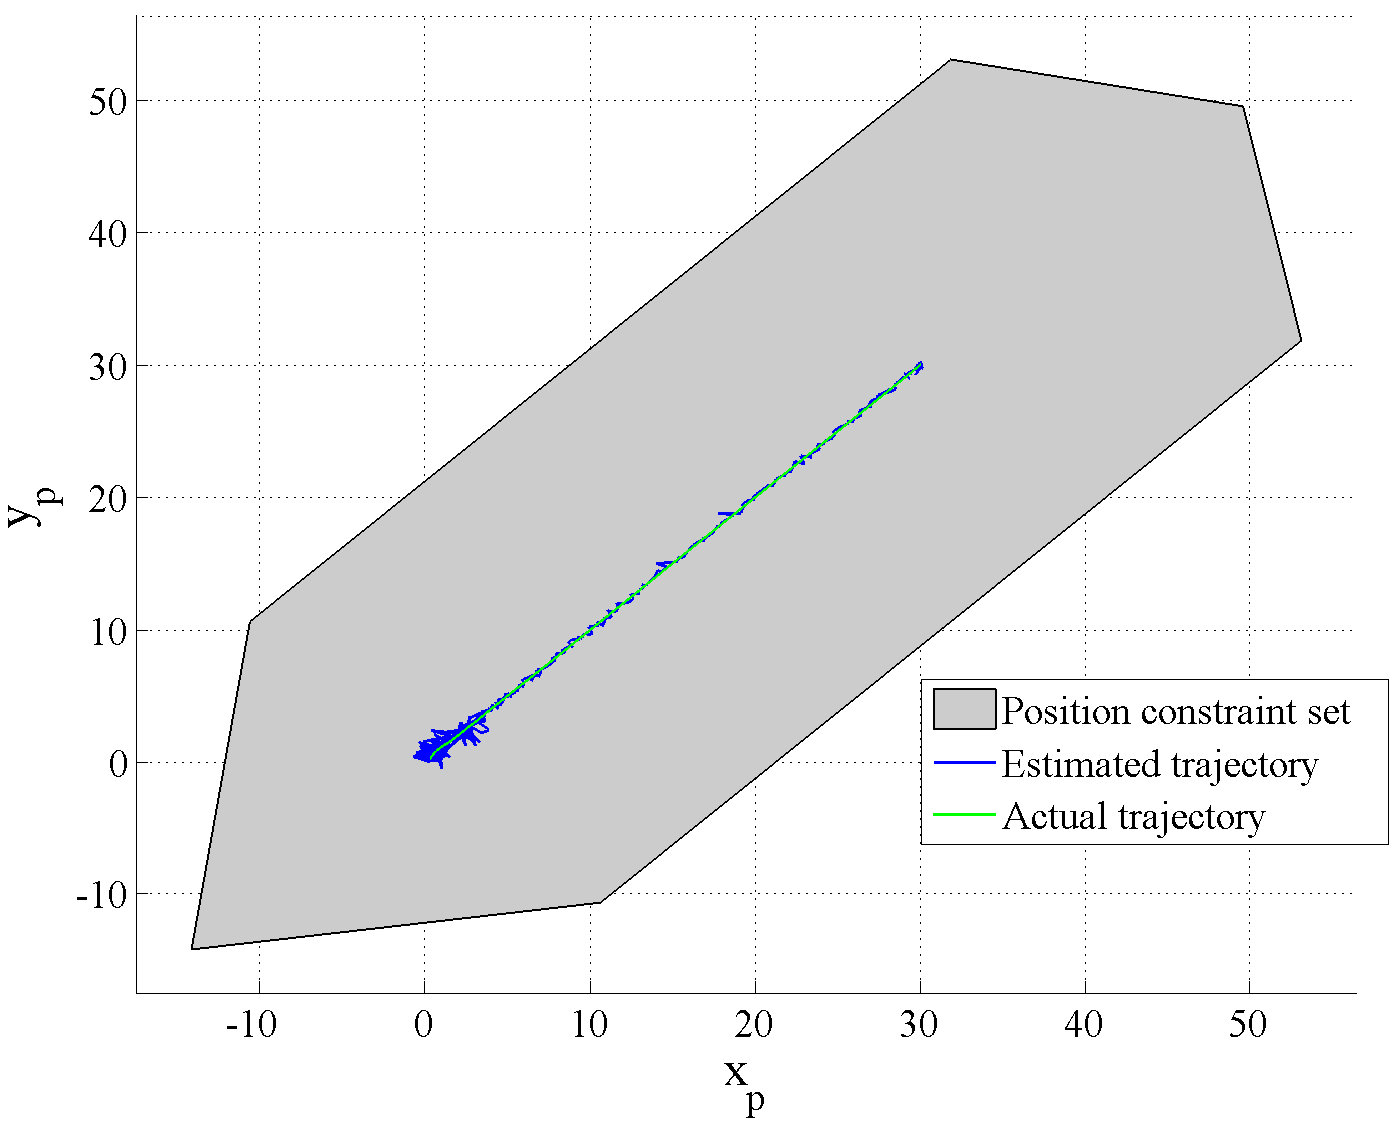
\includegraphics[width=0.8\columnwidth]{figs/TrackingTrajectory_scissored.pdf}
  \caption{Trajectory and safe set of positions.}
  \label{fig:TrackingTrajectory_scissored}
\end{figure}

\begin{figure}
  \centering
  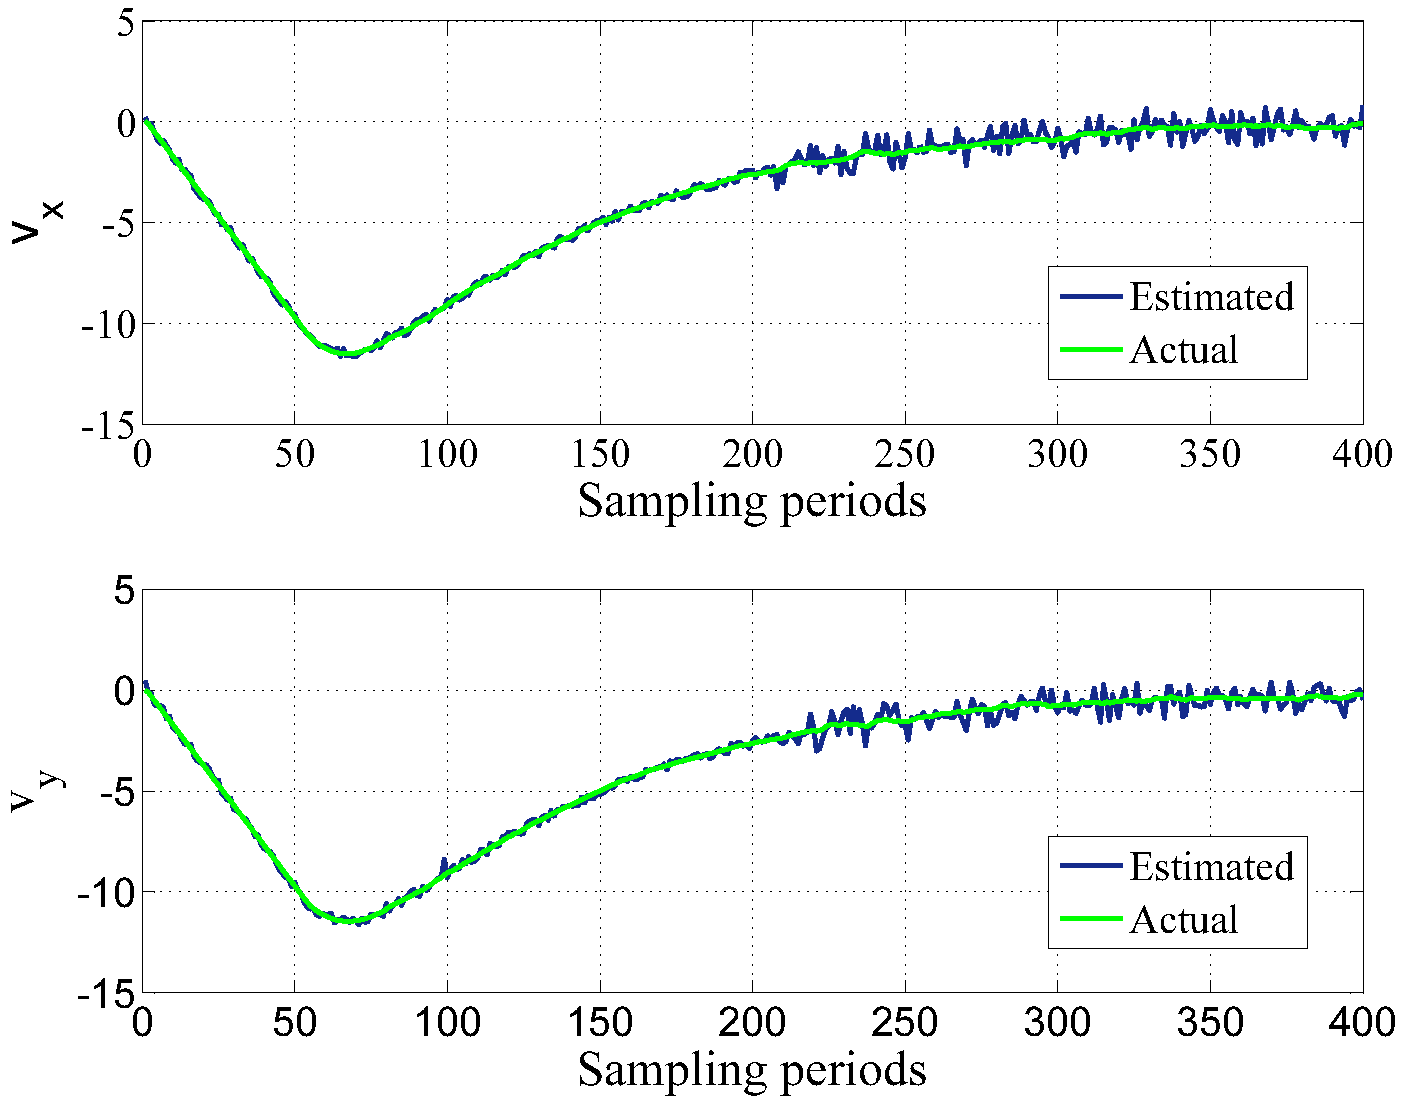
\includegraphics[width=0.80\columnwidth]{figs/velocities_scissored.pdf}
  \caption{Estimated and actual velocities of the vehicle.}
  \label{fig:velocities}
\end{figure}

\begin{figure}
  \centering
  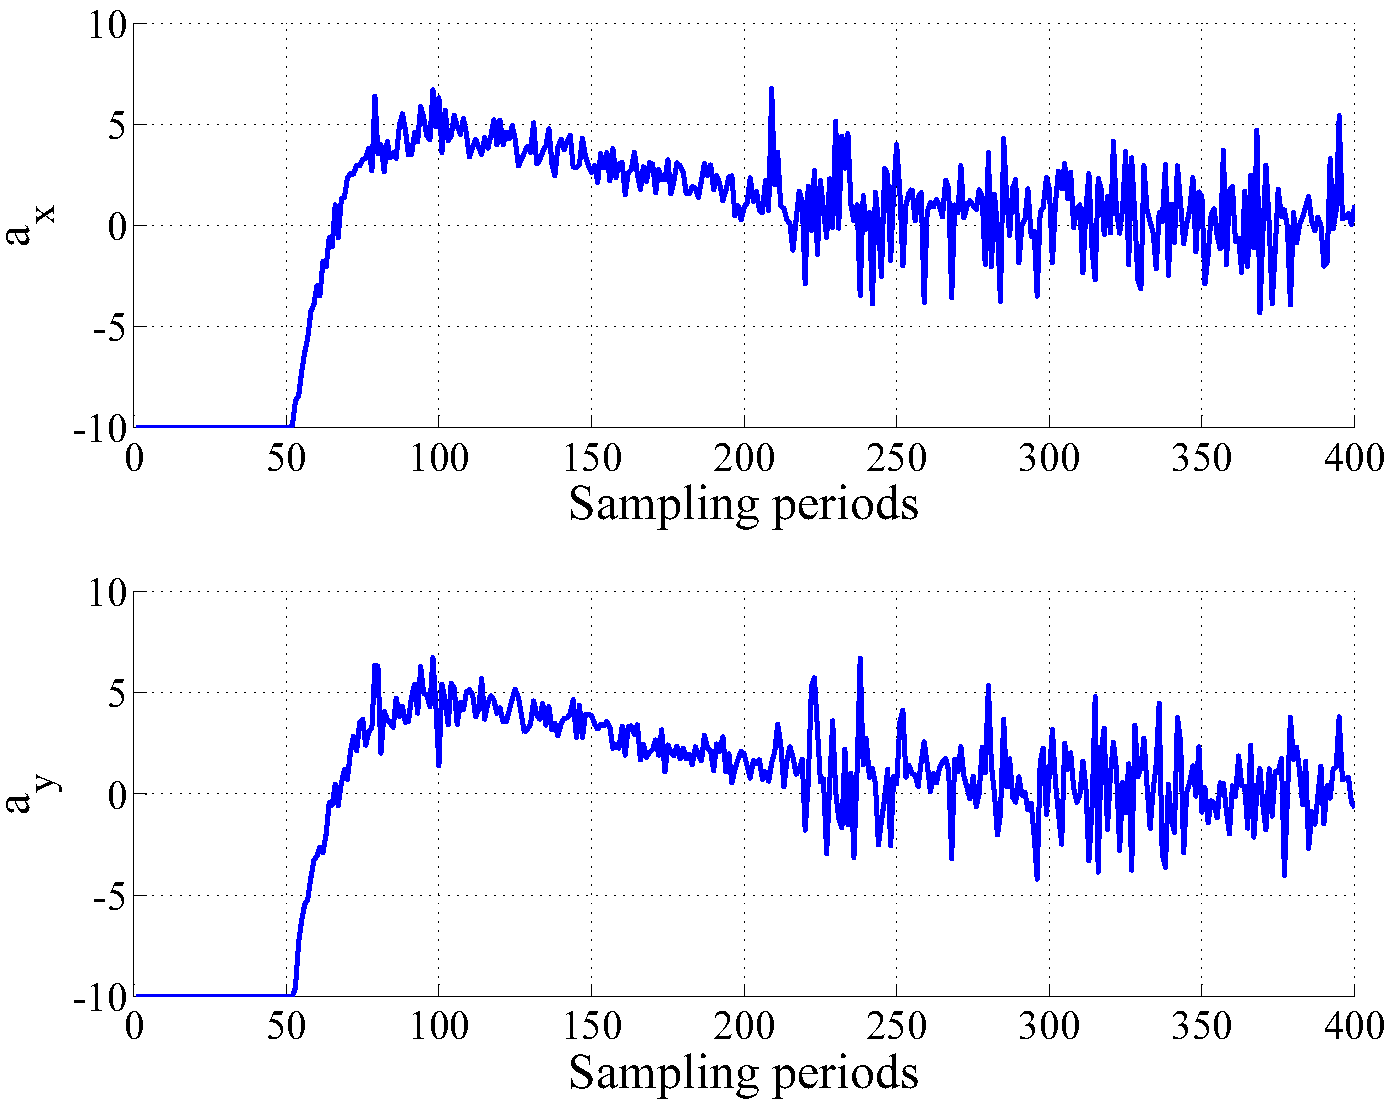
\includegraphics[width=0.80\columnwidth]{figs/inputs_scissored.pdf}
  \caption{Control input (acceleration) to the vehicle.}
  \label{fig:inputs}
\end{figure}

\begin{figure}
  \centering
  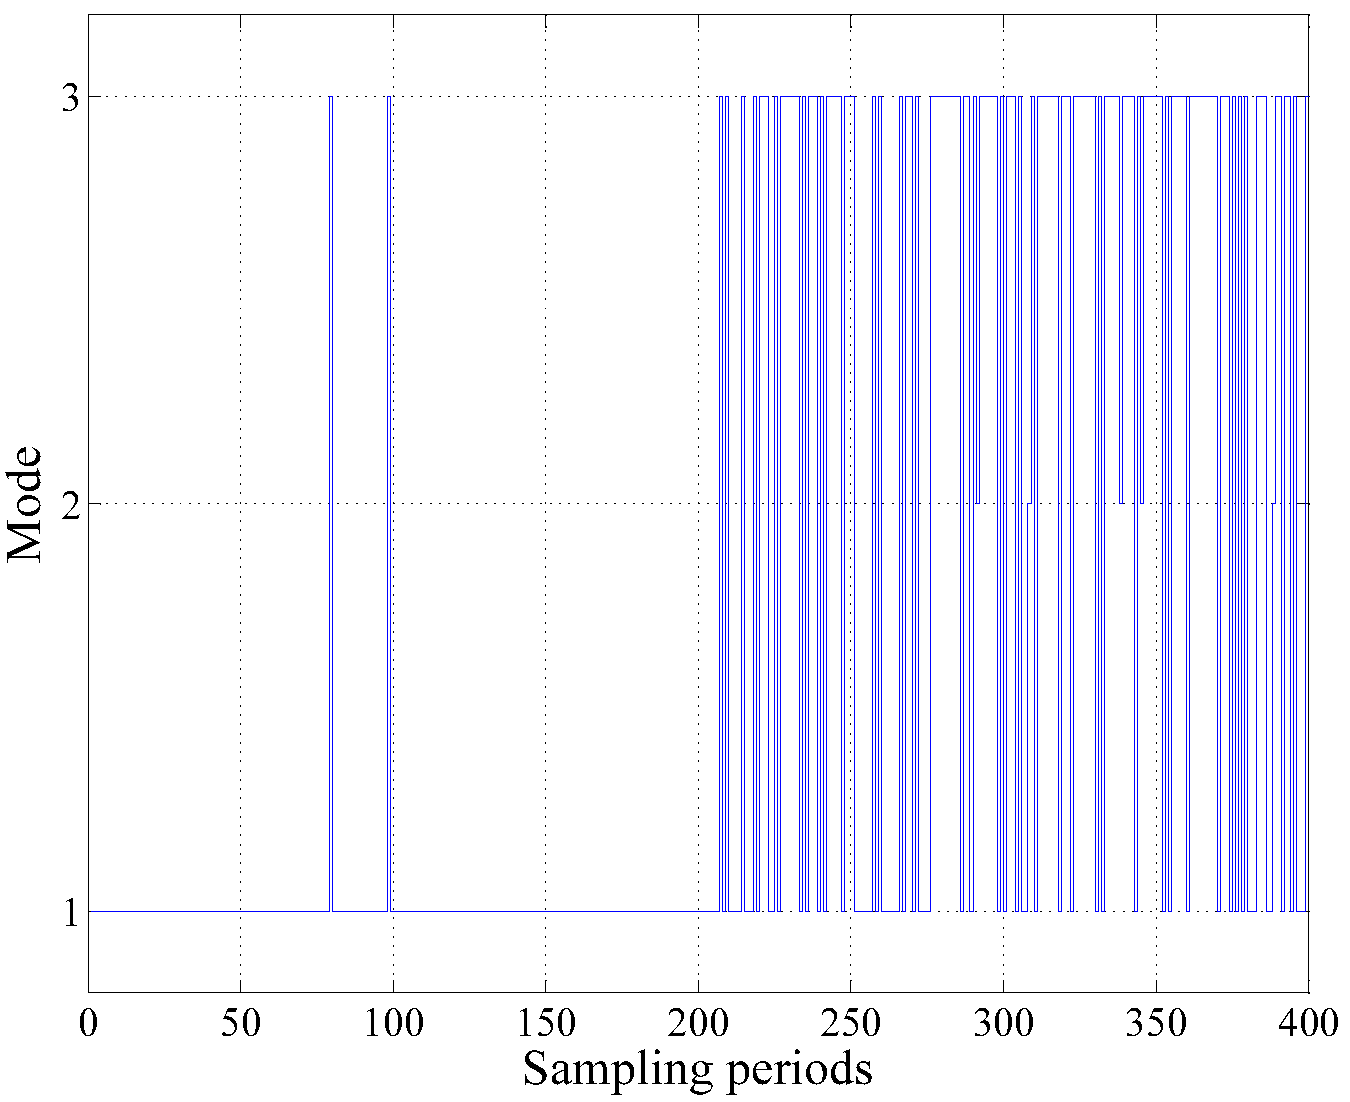
\includegraphics[width=0.9\columnwidth, height=38mm]{figs/ModePicked_scissored.pdf}
  \caption{Estimation mode switching of the proposed control algorithm.}
  \label{fig:modes}
\end{figure}


%%% Local Variables: 
%%% mode: latex
%%% TeX-master: "CDC14_Anytime_Main"
%%% End: 



\section{Conclusions and future work} \label{sec:conclusion}
\section{Conclusions}
%\todo[inline]{use either formulas or formulae consistently}
%\todo[inline]{use {\small } for figure and table captions}
%\todo[inline]{thre's some funny spacing sometimes..}\todo[inline]{use commas in vectors, [2,2,-1] to distinguish the entries}
%\todo[inline]{we present 3 diff control problems, one with and one without control cost. need to make this a bit smoother, right now it's something of a back and forth between the three. (i know, they're special cases of each other, but it reads bad)}
We present a method to obtain smooth (infinity differentiable) approximations to the robustness of MTL formulae, with bounded and asymptotically decaying approximation error. 
Empirically, we show that the approximation is indeed small for a variety of commonly used MTL formulae. 
Through several examples, we show how we leverage the smoothness property of the approximation for solving a control (or falsification) problem by maximizing (or minimizing) the robustness, using SQP, an off-the-shelf gradient descent optimization technique. 
We compare our technique (SR-SQP) to two other approaches for robustness maximization for control of two dynamical systems, with state and input constraints, and show how our approach consistently outperforms the other two and can be used for control of dynamical systems to satisfy an MTL specification.

%\begin{figure}[t]
%\centering
%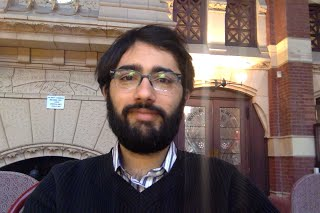
\includegraphics[width=0.49\textwidth]{figures/Habbas}
%\caption{{\small Habbas, pictured here, is the author of this paper, half the papers cited in this paper, half the papers submitted to CPS Week and many others. He can be contacted at habbasATseas.upenn.edu}}
%\label{fig:quad_ssqp}
%\end{figure}


\appendix


%
We will prove the theorem by recursion. We will show that if at any
time step $k$ the RMPC problem $\MPCProb{\sDelay,\sAccu}(\hat{x}_{k},\sDelay[k],\sAccu[k],u_{k-1})$
is feasible and feasible control input $u_{k}=u_{k\Given k}^{\star}$
is applied with estimation mode $\left(\sDelay[k+1],\sAccu[k+1]\right)=\left(\sDelay,\sAccu\right)$
then $u_{k}$ is admissible and at the next time step $k+1$, the
actual plant's state $x_{k+1}$ is inside $\stSet$ and the optimization
$\MPCProb{\sDelay,\sAccu}(\hat{x}_{k+1},\sDelay[k+1],\sAccu[k+1],u_{k})$
is feasible for all disturbances. Then we can conclude the theorem
because, by recursion, feasibility at time step $k_{0}$ implies robust
constraint satisfaction and feasibility at time step $k_{0}+1$, and
so on at all subsequent time steps.

Suppose $\MPCProb{\sDelay,\sAccu}(\hat{x}_{k},\sDelay[k],\sAccu[k],u_{k-1})$
is feasible. Then it has a feasible solution $\left(\{ \overline{z}_{k+j\Given k}^{\star}\} _{j=0}^{N+1},\{ u_{k+j\Given k}^{\star}\} _{j=0}^{N}\right)$
that satisfies all the constraints in \eqref{eq:RMPC1}. Now we will
construct a feasible candidate solution for $\MPCProb{\sDelay,\sAccu}(\hat{x}_{k+1},\sDelay[k+1],\sAccu[k+1],u_{k})$
at the next time step by shifting the above solution by one step.
Consider the following candidate solution for $\MPCProb{\sDelay,\sAccu}(\hat{x}_{k+1},\sDelay[k+1],\sAccu[k+1],u_{k})$:
\begin{subequations}
\label{eq:proofs:candidate-solution}
\begin{align}
\Nom z_{k+j+1\Given k+1} & =\Nom z_{k+j+1\Given k}^{\star}+L_{j}\hat{F}\hat{w}_{k}\label{eq:proofs:candidate-solution:zj}\\
\Nom z_{k+N+2\Given k+1} & =\hat{A}\left(\sDelay\right)\Nom z_{k+N+1\Given k+1}+\hat{B}\left(\sDelay\right)u_{k+N+1\Given k+1}\label{eq:proofs:candidate-solution:zN}\\
u_{k+i+1\Given k+1} & =u_{k+i+1\Given k}^{\star}+K_{i}\left(\sDelay\right)L_{i}\hat{F}\hat{w}_{k}\label{eq:proofs:candidate-solution:uj}\\
u_{k+N+1\Given k+1} & =\kappa\left(\Nom z_{k+N+1\Given k+1}\right)\label{eq:proofs:candidate-solution:uN}
\end{align}
\end{subequations} in which
$j\in\left\{ 0,\dots,N\right\} $, $i\in\left\{ 0,\dots,N-1\right\} $,
and $\kappa\left(\cdot\right)$ is the feedback control law for the
invariant set $\Cc(\sDelay,\sAccu)$ that is used in the terminal
set. We first show that the input and
state constraints are satisfied for $u_{k}$ and $x_{k+1}$, then
we will prove the feasibility of the above candidate solution for
$\MPCProb{\sDelay,\sAccu}(\hat{x}_{k+1},\sDelay[k+1],\sAccu[k+1],u_{k})$.

\noindent\textit{Validity of the applied input and the next state:}
%
The next plant's state is 
\begin{align*}
x_{k+1} & =Ax_{k}+B_{1}\left(\sDelay[k]\right)u_{k-1}+B_{2}\left(\sDelay[k]\right)u_{k}+w_{k}\\
 & =A\left(\hat{x}_{k}+e_{k}\right)+B_{1}\left(\sDelay[k]\right)u_{k-1}+B_{2}\left(\sDelay[k]\right)u_{k\Given k}^{\star}+w_{k}\\
 & =\begin{bmatrix}A & B_{1}\left(\sDelay[k]\right)\end{bmatrix}\begin{bmatrix}\hat{x}_{k}\\
u_{k-1}
\end{bmatrix}+B_{2}\left(\sDelay[k]\right)u_{k\Given k}^{\star} \\
&\qquad\qquad + e_{k+1}+\left(w_{k}+Ae_{k}-e_{k+1}\right)
\end{align*}
in which $e_{k+1}\in\ESet\left(\sAccu\right)$ and $\left(w_{k}+Ae_{k}-e_{k+1}\right)\in\hWc\left(\sAccu[k],\sAccu\right)$.
Note that $\Nom z_{k\Given k}^{\star}=\left[\hat{x}_{k}^{T},u_{k-1}^{T}\right]^{T}$.
Hence we have
\begin{align*}
\begin{bmatrix}x_{k+1}\\
u_{k}
\end{bmatrix} & =\hat{A}(\sDelay[k])\Nom z_{k\Given k}^{\star}+\hat{B}(\sDelay[k])u_{k\Given k}^{\star}\\
&\qquad\qquad +\hat{F}e_{k+1}+\hat{F}\left(w_{k}+Ae_{k}-e_{k+1}\right)\\
 & =\Nom z_{k+1\Given k}^{\star}+\hat{F}e_{k+1}+\hat{F}\left(w_{k}+Ae_{k}-e_{k+1}\right)
\end{align*}
where we use the dynamics in \eqref{eq:RMPC1-dyn}. From \eqref{eq:RMPC1-zset}
and \eqref{eq:RMPC1-Z}, $\Nom z_{k+1\Given k}^{\star}$ satisfies $\Nom z_{k+1\Given k}^{\star}\in\ZSet_{1}\left(\sAccu[k],\sAccu\right)=\ZSet\ominus\hat{F}\ESet\left(\sAccu\right)\ominus\hat{F}\hWc\left(\sAccu[k],\sAccu\right)$.
It follows that
\(
\left[ x_{k+1}^{T}, u_{k}^{T} \right]^{T} \in \ZSet = \stSet\times\inpSet\text{,}
\)
% which allows us to conclude that
therefore  $x_{k+1}\in\stSet$ and $u_{k}\in\inpSet$.


\noindent\textit{Initial condition:}
%
We have from \eqref{eq:estimator-std-dynamics} that $\hat{z}_{k+1}=\hat{A}(\sDelay[k])\hat{z}_{k}+\hat{B}(\sDelay[k])u_{k}+\hat{F}\hat{w}_{k}$.
On the other hand, by \eqref{eq:proofs:candidate-solution:zj},
\begin{align*}
\Nom z_{k+1\Given k+1} & =\Nom z_{k+1\Given k}^{\star}+L_{0}\hat{F}\hat{w}_{k}\\
 & =\hat{A}(\sDelay[k])\Nom z_{k\Given k}^{\star}+\hat{B}(\sDelay[k])u_{k\Given k}^{\star}+L_{0}\hat{F}\hat{w}_{k}\text{.}
\end{align*}
Note that $\Nom z_{k\Given k}^{\star}=\hat{z}_{k}$, $u_{k}=u_{k\Given k}^{\star}$,
and $L_{0}=\IdentityMatrix$. Therefore $\Nom z_{k+1\Given k+1}=\hat{z}_{k+1}$,
hence the initial condition is satisfied.


\noindent\textit{Dynamics:}
%
We show that the candidate solution satisfies the dynamics constraint
in \eqref{eq:RMPC1-dyn}. For $0\leq j<N$ we have
\begin{align*}
&\Nom z_{k+j+2\Given k+1} \\
=\, & \Nom z_{k+j+2\Given k}^{\star}+L_{j+1}\hat{F}\hat{w}_{k}\\
=\, &\hat{A}\left(\sDelay\right)\Nom z_{k+j+1\Given k}^{\star}+\hat{B}(\sDelay)u_{k+j+1\Given k}^{\star}+L_{j+1}\hat{F}\hat{w}_{k}\\
=\, &\hat{A}\left(\sDelay\right)\left(\Nom z_{k+j+1\Given k+1}-L_{j}\hat{F}\hat{w}_{k}\right) \\
&+\hat{B}(\sDelay)\left(u_{k+j+1\Given k+1}-K_{j}\left(\sDelay\right)L_{j}\hat{F}\hat{w}_{k}\right) +L_{j+1}\hat{F}\hat{w}_{k} \\
=\, &\hat{A}\left(\sDelay\right)\Nom z_{k+j+1\Given k+1}+\hat{B}(\sDelay)u_{k+j+1\Given k+1} \\
&-\left(\hat{A}\left(\sDelay\right) + \hat{B}(\sDelay)K_{j}\left(\sDelay\right)\right)L_{j}\hat{F}\hat{w}_{k}+L_{j+1}\hat{F}\hat{w}_{k}\\
=\, &\hat{A}\left(\sDelay\right)\Nom z_{k+j+1\Given k+1}+\hat{B}(\sDelay)u_{k+j+1\Given k+1}
\end{align*}
where the equality in \eqref{eq:RMPC1-Lj} is used to derive the last
equality. % from the previous one.
Therefore the dynamics constraint
is satisfied for all $0\leq j<N$. For $j=N$, the constraint is satisfied
by construction by \eqref{eq:proofs:candidate-solution:zN}.


\noindent\textit{State constraints:}
%
We need to show that $\Nom z_{(k+1)+j\Given k+1}\in\ZSet_{j}\text{\ensuremath{\left(\sAccu,\sAccu\right)}}$
for all $j\in\left\{ 0,\dots,N\right\} $. Consider any $0\leq j<N$.
\eqref{eq:RMPC1-Zj} states that $\ZSet_{j+1}\left(\sAccu[k],\sAccu\right)=\ZSet_{j}\left(\sAccu,\sAccu\right)\ominus L_{j}\hat{F}\hWc\left(\sAccu[k],\sAccu\right)$.
From the construction of the candidate solution we have $\Nom z_{k+j+1\Given k+1}=\Nom z_{k+j+1\Given k}^{\star}+L_{j}\hat{F}\hat{w}_{k}$,
where $\hat{w}_{k}\in\hWc\left(\sAccu[k],\sAccu\right)$ and $\Nom z_{k+j+1\Given k}^{\star}\in\ZSet_{j+1}\left(\sAccu[k],\sAccu\right)$.
By definition of the Pontryagin difference, we conclude that $\Nom z_{k+j+1\Given k+1}\in\ZSet_{j}\left(\sAccu,\sAccu\right)$
for all $j\in\left\{ 0,\dots,N-1\right\} $.

At $j=N$ the candidate solution in \eqref{eq:proofs:candidate-solution:zj}
gives us $\Nom z_{(k+1)+N\Given k+1}=\Nom z_{k+N+1\Given k}^{\star}+L_{N}\hat{F}\hat{w}_{k}$.
Because $\Nom z_{k+N+1\Given k}^{\star}\in\ZSet_{f}\left(\sAccu[k],\sAccu\right)=\Cc\left(\sDelay,\sAccu\right)\ominus L_{N}\hat{F}\hWc\left(\sAccu[k],\sAccu\right)$
and $\hat{w}_{k}\in\hWc\left(\sAccu[k],\sAccu\right)$, we have
$\Nom z_{(k+1)+N\Given k+1}\in\Cc\left(\sDelay,\sAccu\right)$. The
definition of $\Cc\left(\sDelay,\sAccu\right)$ in \eqref{eq:RMPC1-Zf-invariant}
implies $\Cc\left(\sDelay,\sAccu\right)\subseteq\ZSet_{N}\left(\sAccu,\sAccu\right)$.
Therefore $\Nom z_{(k+1)+N\Given k+1}\in\ZSet_{N}\left(\sAccu,\sAccu\right)$.


\noindent\textit{Terminal constraint:}
%
We need to show that $\Nom z_{k+N+2\Given k+1}\in\ZSet_{f}\left(\sAccu,\sAccu\right)=\Cc\left(\sDelay,\sAccu\right)\ominus L_{N}\hat{F}\hWc\left(\sAccu,\sAccu\right)$.
Add $L_{N}\hat{F}\hat{w}$, for any $w\in\hWc\left(\sAccu,\sAccu\right)$,
to both sides of \eqref{eq:proofs:candidate-solution:zN} and note that
$u_{k+N+1\Given k+1}=\kappa\left(\Nom z_{k+N+1\Given k+1}\right)$,
we have 
\begin{multline*}
  \Nom z_{k+N+2\Given
    k+1}+L_{N}\hat{F}\hat{w}=\hat{A}\left(\sDelay\right)\Nom
  z_{k+N+1\Given k+1} \\
  +\hat{B}\left(\sDelay\right)\kappa\left(\Nom
    z_{k+N+1\Given k+1}\right)+L_{N}\hat{F}\hat{w}\text{.}
\end{multline*}


 It follows from $\Nom z_{k+N+1\Given k+1}\in\Cc\left(\sDelay,\sAccu\right)$
and from the definition of the invariant control invariant admissible
set $\Cc\left(\sDelay,\sAccu\right)$ 
that $\Nom z_{k+N+2\Given k+1}+L_{N}\hat{F}\hat{w}\in\Cc\left(\sDelay,\sAccu\right)$
for all $w\in\hWc\left(\sAccu,\sAccu\right)$. Then by definition
of the Pontryagin difference, we conclude that $\Nom z_{k+N+2\Given k+1}\in\Cc\left(\sDelay,\sAccu\right)\ominus L_{N}\hat{F}\hWc\left(\sAccu,\sAccu\right)=\ZSet_{f}\left(\sAccu,\sAccu\right)$.


%%% Local Variables: 
%%% mode: latex
%%% TeX-master: "CDC14_Anytime_Main"
%%% End: 


% 
% The following two commands are all you need in the
% initial runs of your .tex file to
% produce the bibliography for the citations in your paper.
%\vspace{-6pt}

\bibliographystyle{IEEEtran}
\bibliography{IEEEabrv,anytime_ref}
%\bibliography{IEEEabrv,references,Case_bib}  % sigproc.bib is the name of the Bibliography in this case

% You must have a proper ".bib" file
%  and remember to run:
% latex bibtex latex latex
% to resolve all references
%
%APPENDICES are optional
%\balancecolumns
%\appendix

%Appendix A
% \section*{Appendix}
% \label{sec:proofs}



\end{document}


%%% Local Variables: 
%%% mode: latex
%%% TeX-master: t
%%% End: 
